\documentclass{article}[a4paper,12pt]
\usepackage[utf8]{inputenc}
\usepackage{amsmath,amssymb,amsthm,amsfonts,mathtools}
\usepackage[inline]{enumitem}
\usepackage{soul}
\usepackage{cancel}
\usepackage{hyperref}
\usepackage{centernot}
\usepackage{pifont}
\usepackage{changepage}
\usepackage{subcaption}
\usepackage[section]{placeins}
\usepackage{lipsum, graphicx, caption}
\usepackage{float}
\usepackage{commath}
\usepackage{wrapfig}
\usepackage{amsmath}
\usepackage{amsfonts}
\usepackage{amssymb}
\theoremstyle{definition}
\newtheorem{innercustomgeneric}{\customgenericname}
\providecommand{\customgenericname}{}
\newcommand{\newcustomtheorem}[2]{%
  \newenvironment{#1}[1]
  {%
   \renewcommand\customgenericname{#2}%
   \renewcommand\theinnercustomgeneric{##1}%
   \innercustomgeneric
  }
  {\endinnercustomgeneric}
}
\newcustomtheorem{customthm}{Theorem}
\newcustomtheorem{customlem}{Lemma}
\newcustomtheorem{customdefn}{Definition}
\newcustomtheorem{customprop}{Proposition}
\newcustomtheorem{customexer}{Exercise}
\renewcommand{\qedsymbol}{$\blacksquare$}

\setlength\parindent{0pt}
\let\emptyset\varnothing
\usepackage{geometry}
\geometry{
	a4paper, portrait,
	total = {170mm,257mm},
	left = 20mm,
	top = 20mm,
}

\usepackage{xcolor}
\usepackage{pagecolor}
\pagecolor{white}
\color{black}

\title{\textbf{Introduction to Game Developement}}
\author{
	\textbf{Om Prabhu}\\
	19D170018\\
	Undergraduate, Department of Energy Science and Engineering\\
	Indian Institute of Technology Bombay\\}
\date{Last updated \today}

\begin{document}
\maketitle
\vspace{-12pt}
\hrulefill
\vspace{6pt}

\textbf{NOTE:} This document is a brief compilation of my notes taken during a course in game design and development. You are free to use it and my project files for your own personal use \& modification. You may check out the course here: \texttt{\href{https://www.coursera.org/learn/game-development?specialization=game-development}{https://www.coursera.org/learn/game-development?specialization=game-development}}.

\hrulefill
\tableofcontents
\vspace{6pt}

\hrulefill
\pagebreak

\section{Introduction}
\subsection{About myself}
Hello. I am Om Prabhu, currently an undergrad at the Department of Energy Science and Engineering, IIT Bombay. If you have gone through my website (\texttt{\href{https://omprabhu31.github.io}{https://omprabhu31.github.io}}) earlier, which is probably where you found this document too, you will know that I love playing video games, story-rich titles in particular. I also listen to a lot of music and engage in a little bit of creative writing as and when I get time. With this brief self-introduction, let's get into what actually motivated me to pursue game development.

\subsection{Motivation}
Most of my motivation for pursuing game development came from playing games itself. I am talking less of titles like \textit{Grand Theft Auto}, generic FPS/RPGs, etc meant purely for self-entertainment and more about games like \textit{Life is Strange}, \textit{When the Darkness Comes}, etc that actually give you some amazing stories and/or simple, powerful messages to be remembered for life. When one has experiences like this, the question naturally hangs at the back of their minds - why not create enriching experiences like this?
\vspace{6pt}

Now while playing games (of all genres) is vital to understanding what essentially makes a good game, they are two very different things - it's like comparing movie binging to actually making movies. Making games involves a lot of hardwork at different stages of the development process and there is a reason why good game developers take their time (often more than 10 years) before putting out a game on the market.
\vspace{6pt}

Nevertheless, I decided to give it a shot - the worst that could happen is I could end up hating it, but I hate it during quarantine anyway.

\hrulefill
\vspace{6pt}

\textbf{NOTE:} 
\begin{enumerate}
	\item This entire course works with Unity3D as the game engine, however the exact same concepts apply to other engines like Unreal, Godot, etc as well.
	\item Even if you are using a newer or older version of Unity, the concepts apply just as well. In fact, there is almost negligible difference in functionality between releases.
	\item The source files for course projects are available on my website for free use and modification. I will mainly be working with the 2019.4.2f1 and 2017.4.40f1 LTS releases of Unity, so you might need to install these versions of the engine before you try them out.
	\item Most of the project builds will be for the WebGL platform. Many browsers do not support running local WebGL content out of the box. You might find this guide handy: \texttt{\href{techwiser.com/enable-webgl}{techwiser.com/enable-webgl}}
	\item If you want to install Standard Assets through Unity Hub, then you might want to install a 2017 LTS release (Unity no longer releases Standard Assets from 2018). Otherwise there is always the option of importing and using 2017 Standard Assets in a 2018 or 2019 release.
\end{enumerate}
\hrulefill
\pagebreak

\section{Overview of Game Development}
\subsection{Factors to consider before starting out}
\begin{center}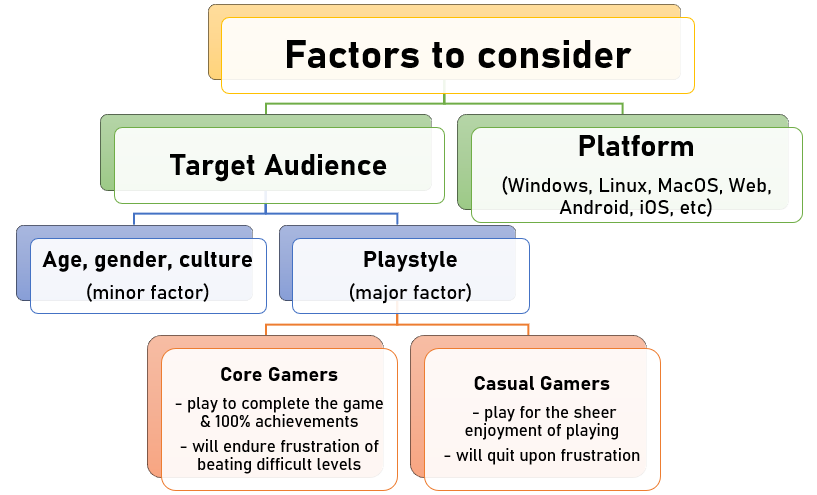
\includegraphics[scale=0.8]{gamedev_basic_factors_to_consider.png}\end{center}

\subsection{Hierarchy of game structure}
Keeping in mind the above factors, we proceed to conceptualize the game structure.
\begin{center}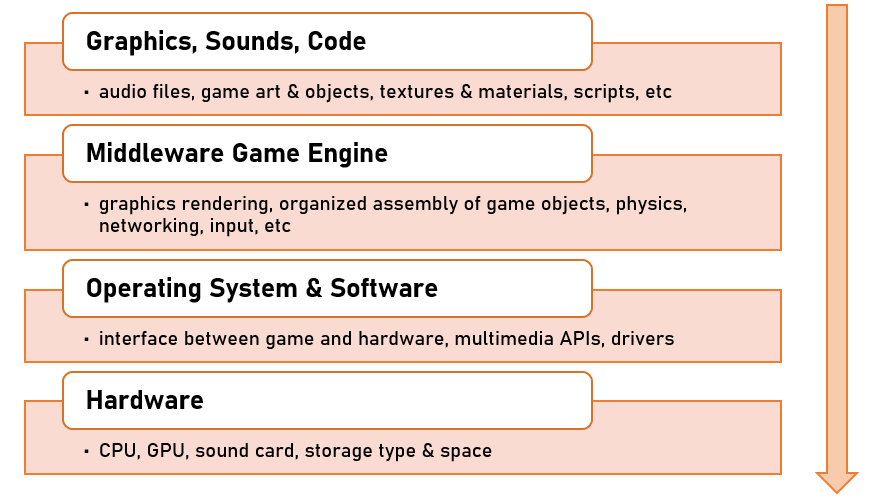
\includegraphics[scale=0.8]{game_design_hierarchy.png}\end{center}

While normally we would construct anything from the ground up, from a game design perspective things work better when conceptualized from the top down. 
\begin{itemize}
	\item We first create everything essential, i.e. `game assets' - that would mean any art, textures \& materials, game object models, audio/music and scripts (basically code that defines interaction between objects)
	\item Then, we actually construct the levels in the game using the above created assets in an engine like Unity, Unreal, Godot, etc
	\item We then build the game for the intended platforms
	\item Finally the game is tested for bugs and to determine the requirements for a system that could hope to run our game
\end{itemize}

\subsection{Team structure and roles}
Considering all the stuff from the previous subsection, it would be near impossible for a single person to carry out all the work required and make an end product that ticks all the boxes (individual developers do exist still). This is why there are often teams, ranging in size from as small as 2-3 people to well over 1000 employees, with each member having one or more roles to perform.
\begin{itemize}
	\item Game Designer: execution of the idea behind the story, designing levels, gameplay mechanics, organizing assets and documents
	\item Story Designer: character design, story arcs, writing dialogues, etc
	\item Game Producer: monitoring project budgets, keeping track of deadlines, keeping the team together
 	\item Programmer: writing actual code to determine how game objects interact
	\item Game Artist: create concept art, textures for game objects to give them unique looks 
	\item Sound Designer: create and edit music to match the mood of various in-game scenes
	\item Game Tester: not the same as a player; requires sitting on a single game level for hours to identify bugs/inconsistencies
\end{itemize}
Depending on the size of the team, each person may assume one or more of the above roles based on what they can best do:
\begin{itemize}
	\item a small team (1-5 people) may be able to make do with just general purpose designers, artists and programmers, and each person will be more or less actively involved in production work
	\item a medium sized team (6-25 people) may additionally require a manager/producer and specialized designers \& artists
	\item a large team (25+ people) will have supplementary roles like scripters (people who have knowledge of programming as well as design), technical artists (programmers who can also work as artists) and level designers (who make the artwork and game design for separate levels)
\end{itemize}
\hrulefill
\pagebreak

\section{The Unity3D Engine}
All games need a few basic features - loading and displaying game assets, playing sound FX. receive player input and react to it, some code to define game rules and mechanics. One way to incorporate all of this is to build everything from scratch i.e. the core game software, renderers, etc. While this can certainly be done, it is much easier to use a game engine to do most of the work for us.
\vspace{6pt}

A game engine is a platform that provides basic game functionality, support for integration of game objects of multiple different formats. This allows us to focus on the actual unique gameplay elements.
\vspace{6pt}

Some advantages of using the Unity3D game engine are:
\begin{itemize}
 	\item great documentation (by which I mean insanely great) and a very large dev community
	\item very fast build times and support for many platforms
	\item great asset pipeline (mechanism to import and use game assets)
	\item not as processor intensive as other engines like Unreal
	\item can actively switch between different editor versions using Unity Hub without needing to rebuild the entire project
\end{itemize}
\textbf{NOTE:} If you take up this course, the instructor will mention that Unity3D offers flexibility in programming languages between C\# and JavaScript. This is no longer valid after the 2019 LTS releases. However, many .NET compatible languages like C++ can be used if they are first compiled into a DLL (for which you can refer this - \texttt{\href{https://docs.unity3d.com/Manual/UsingDLL.html}{https://docs.unity3d.com/Manual/UsingDLL.html}}).
\subsection{Unity3D interface and configuration}
The process of downloading and installing Unity is very intuitive and I won't go over it. However, note that Unity has stopped distributing the Standard Assets Example Project from 2018 onwards, so you might need to use the 2017 releases if you want to try stuff out with the example project. On launching Unity, the editor window might look something similar to this:
\vspace{6pt}

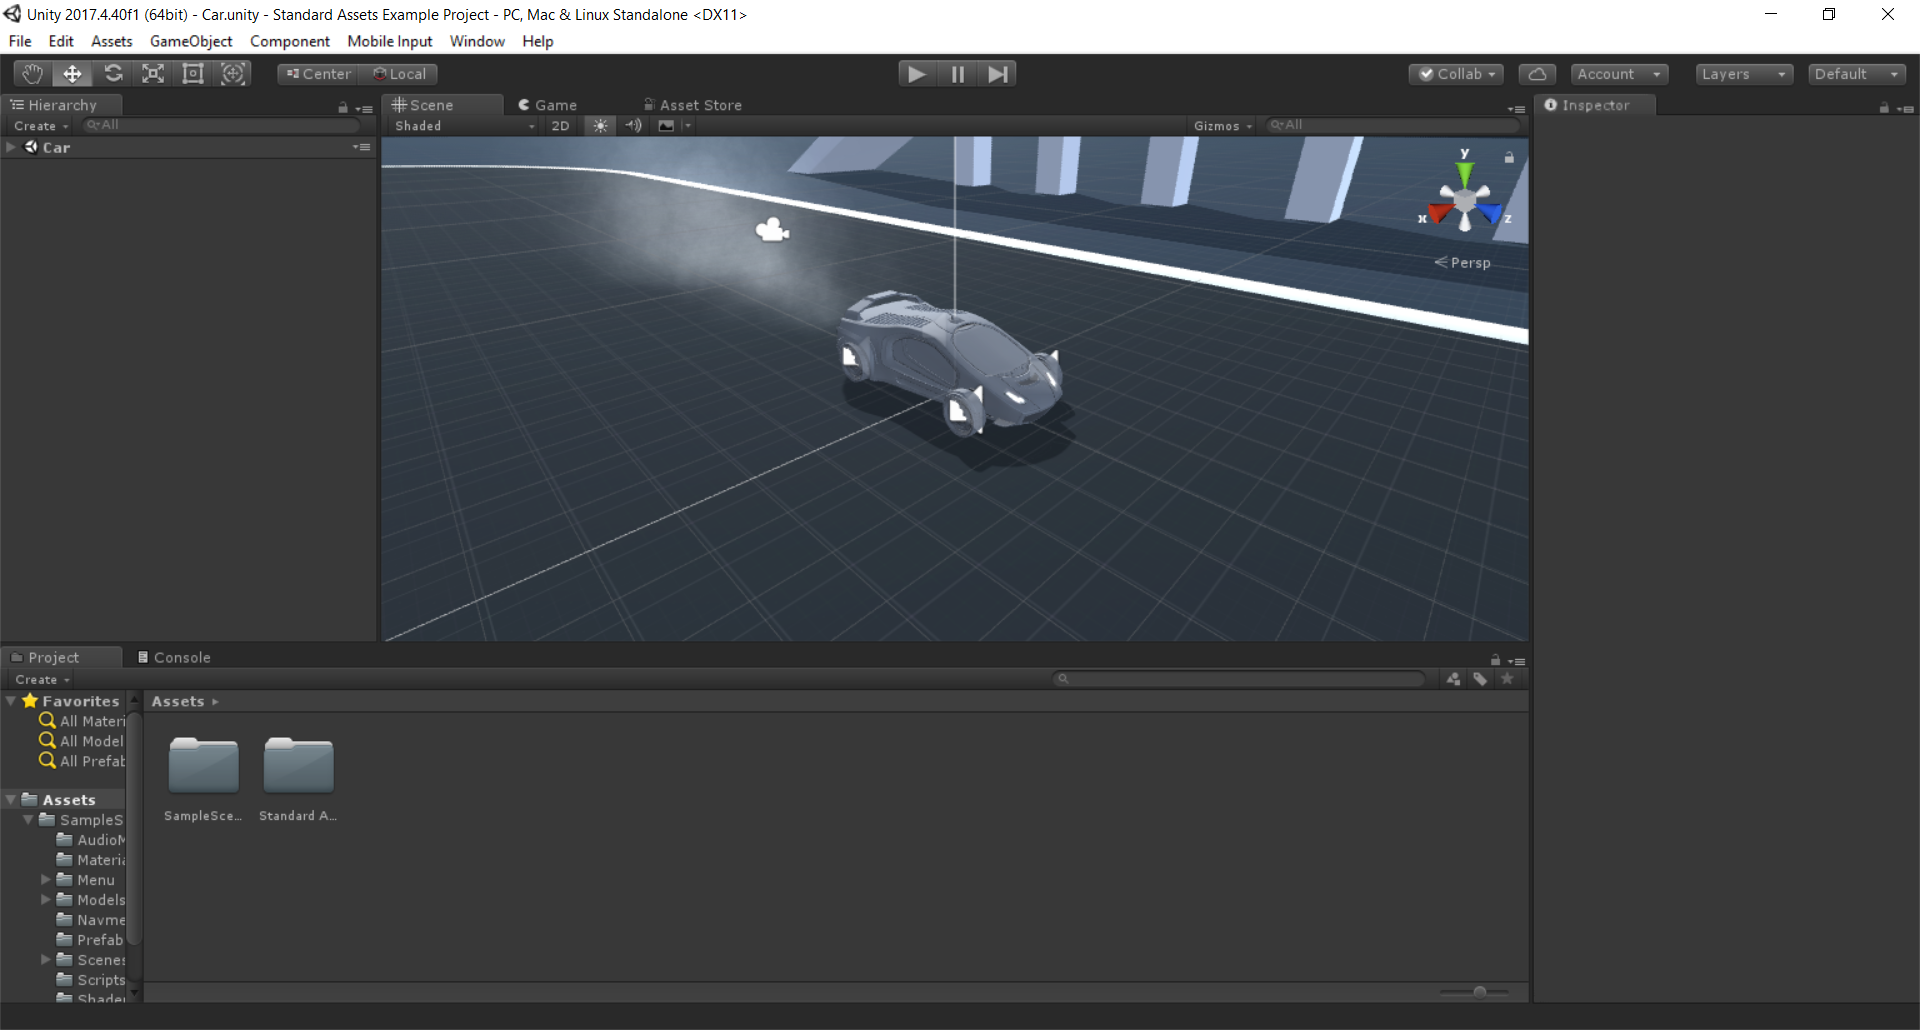
\includegraphics[width=\textwidth]{unity_default_layout.png}
\vspace{1pt}

I personally hate this layout (for the main reason that you can only see 4 panels at any given time which means you have to keep on switching between tabs). You can play around with this layout by simply dragging various tabs around the window to get the window configuration you like. I personally prefer this editor configuration, since now you can see all tabs within a single window:

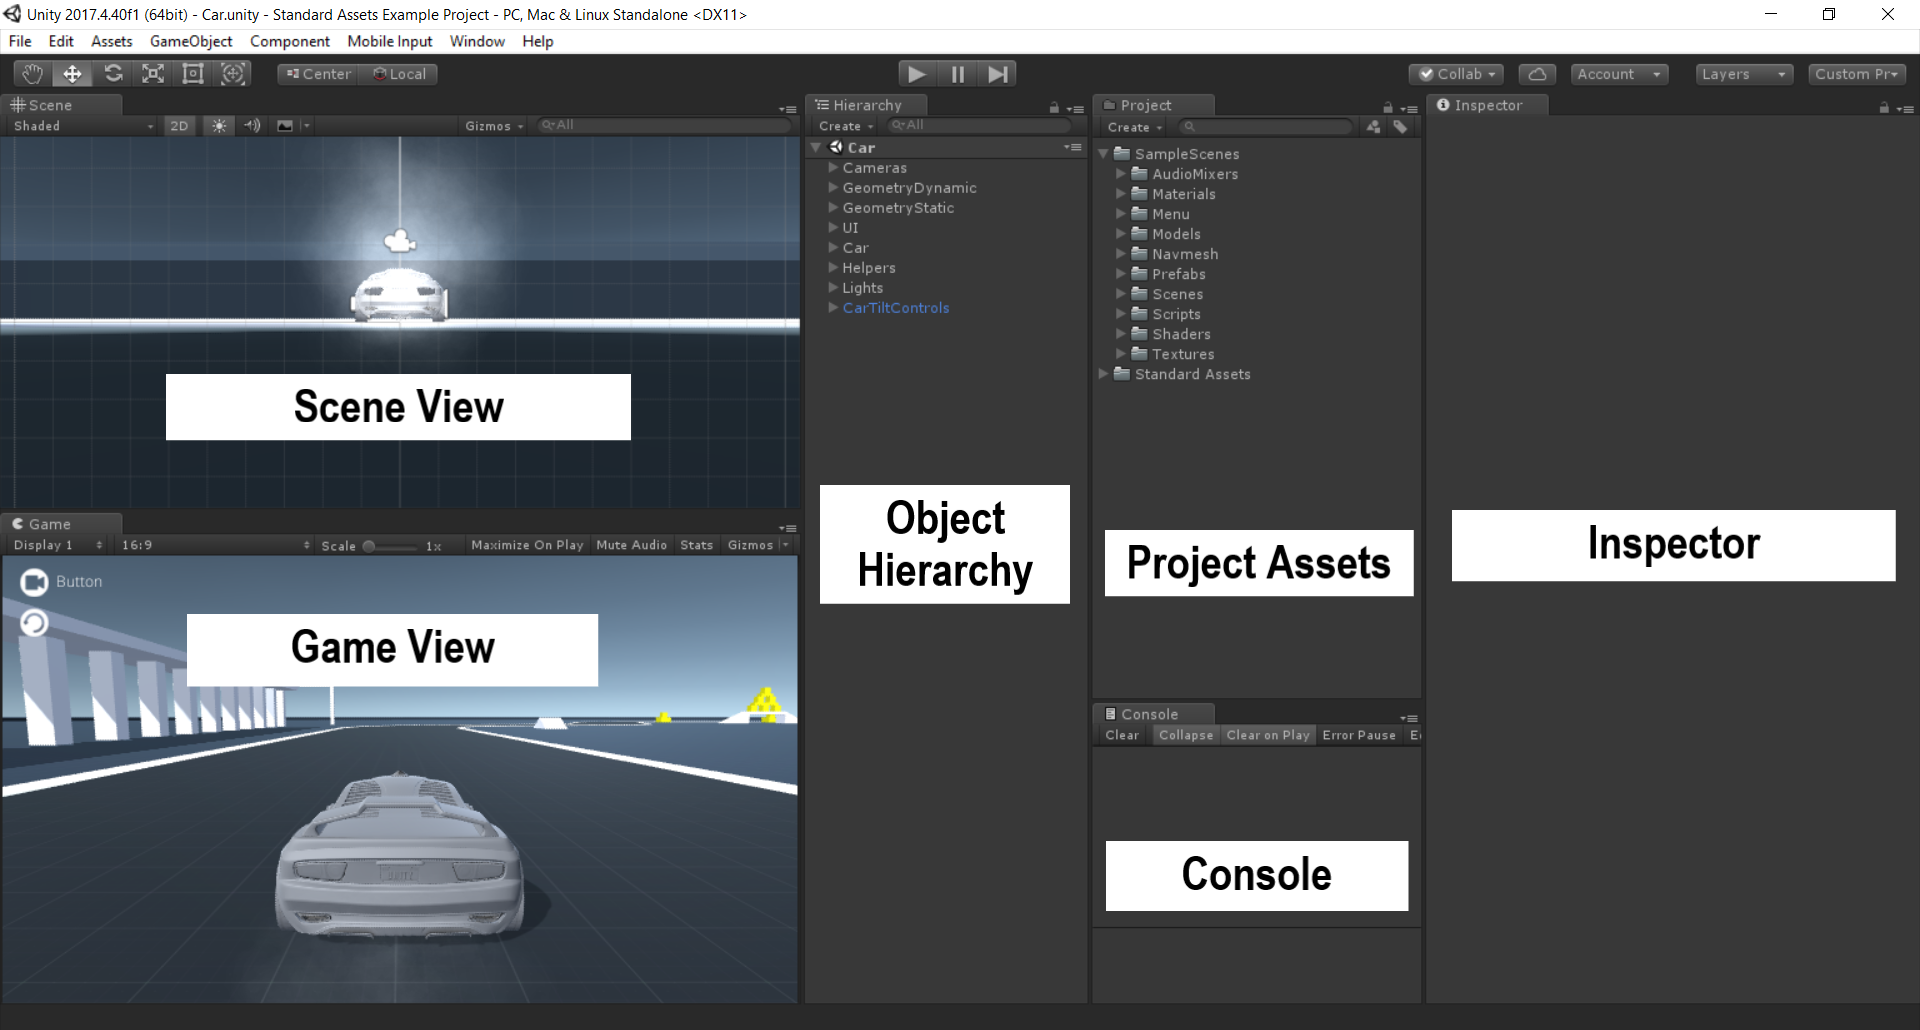
\includegraphics[width=\textwidth]{unity_custom_layout.png}
\vspace{1pt}

Let us now take a brief look at the various elements in the Unity3D interface:
\begin{itemize}
	\item Scene View: visual level editor for the currently open scene (edit mode)
	\item Game View: shows the view through the active camera object (the play button can be used to switch to play mode for playing and testing the game within the Unity editor)
	\item Object Hierarchy: hierarchical list of all game objects being used in the current scene along with parent-child relationships (is linked directly to the scene view)
	\item Project Assets: all the files and folders that make up the project (including the ones which are not being used in the current scene, but can be used later)
	\item Console: displays errors while building the scene (eg: lighting needs to be rebaked)
	\item Inspector: shows details of all game objects and components (like position, scale, scripts, materials, audio, etc) attached to them
\end{itemize}
You might now want to explore the Unity editor to look at various features. There are also many quick shortcuts in Unity that you can refer to here: \texttt{\href{https://docs.unity3d.com/Manual/UnityHotkeys.html}{https://docs.unity3d.com/Manual/UnityHotkeys.html}}.
\vspace{6pt}

\textbf{NOTE:} If you ever need to move/rename/delete asset files, do it in the Unity editor itself (in the Project panel) and \textit{NOT} in the system file explorer - doing this may affect some connections between game objects and break your project.

\hrulefill
\pagebreak
\section{Basic Concepts}
\subsection{Game graphics concepts}
Before we start using Unity, let us briefly discuss the basics of computer graphics using the graphics display model:

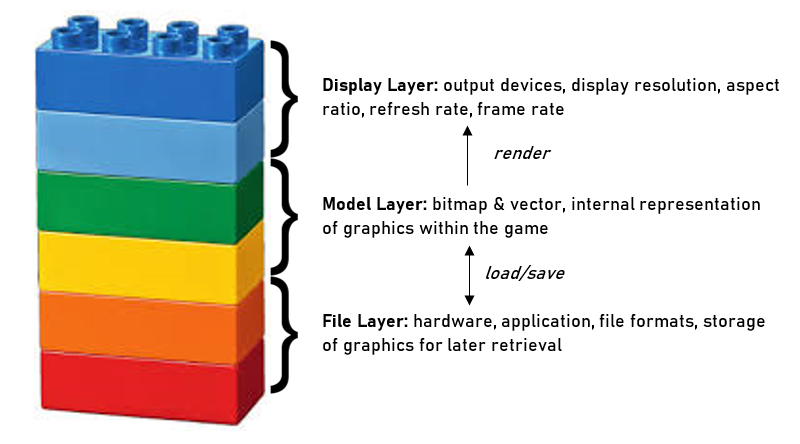
\includegraphics[width=\textwidth]{graphics_concepts.png}
\begin{enumerate}
	\item Display layer:
	\begin{itemize}
		\item display devices: laptop, smartphone, tablet, VR glasses
		\item display resolution: measure of how accurately a display approximates continuous images using finite pixels (pixel dimensions like 1920$\times$1080, dots/pixels per inch)
		\item aspect ratio: proportion of pixel map width vs height (eg: 1920$\times$1080 and 1280$\times$720 both have aspect ratio of 16:9)
		\item refresh rate: maximum rate at which the hardware can refresh the display image (expressed in hertz)
		\item frame rate: actual rate at which the hardware updates the display images (eg: a complex game might run at 60 FPS even though the display has a refresh rate of 240 Hz)
	\end{itemize}
	\item Model layer:
	\begin{itemize}
		\item bitmap image: stores color information about each individual pixel (zooming degrades image quality since we are not creating new pixels, but rather zooming in on the available pixels)
		\item vector image: stored internally as mathematical equations representing certain geometric aspects of the image (can be scaled up without loss of quality)
		\item vector images take longer to load (additional step of converting vector information to the corresponding pixel map before rendering it to the display), hence usually give lower frame rates
		\item 3D graphics: essentially vector graphics in 3 dimensions (i.e. 3D model defined by geometric polygons, usually triangles, to create a `mesh' of the model) - for realtime rendering at high FPS, we use low polygon modeling (i.e. limit number of polygons)
	\end{itemize}
	\item File layer:
	\begin{itemize}
		\item Unity supports nearly all file formats (support for 2D vector graphics also added recently)
		\item for 3D formats (eg: native Maya, 3ds Max, Blender files), Unity converts to FBX files while importing
	\end{itemize}
\end{enumerate}
\textbf{NOTE:} As a general rule of thumb, try to maintain highest achievable image quality for as long as possible - reduce it only if it is adversely affecting the gameplay.
\pagebreak
\subsection{Game audio concepts}
We can apply the analogy of the graphics display model here as well:
\begin{itemize}
	\item instead of the display we have a device which converts digital data signals back into analogue waves (7.1 surround system, headphones, etc)
	\item instead of image storage algorithms we have a process called sampling (approximation of continuous analogue input to discrete digital pulses)
	\item sample rate: number of times per second the sound wave is `sampled' (typically 44.1 kHz)
	\item sample size: amount of data stored per sample (typically 8, 16 or 32 bits)
	\item typical file formats include WAV, AIFF, OGG, MP3, etc (software like Adobe Audition or Audacity have their native file formats)
\end{itemize}
Audio is very important to games, and also one of the tougher things to actually make or synthesize digitally. There are 3 main types of game audio:
\begin{itemize}
	\item voice: easiest to come by - voice actors need not be professionals, they can be friends, family, etc (pro tip: keep background noise as low as possible, otherwise noise removal is a very difficult task in production)
	\item sound FX:
	\begin{itemize}
		\item[$-$] reactive FX: effects that occur as things happen in the game (royalty free, creative commons licensed effects can be easily found in places like the Unity Asset Store)
		\item[$-$] ambient FX: ambient noises that add a feeling of immersion (natural sounds often work better than digitized ambient effects)
	\end{itemize}
	\item music: adds emotional impact and complements the atmosphere (again free resources exist; commercially produced music will need you to buy a license in order that you do not violate copyright law)
\end{itemize}
\hrulefill
\begin{center}\textbf{END OF WEEK 1}\end{center}
This is the end of the documentation from Week 1 of the course. Continue reading forward, or head over into Unity and try out some stuff yourself. In subsequent weeks, we will be actually making stuff in Unity:
\begin{itemize}
	\item Week 2 - Solar System Simulation
	\item Week 3 - Roller Madness
	\item Week 4 - Box Shooter
\end{itemize}

\hrulefill
\pagebreak
\section{Solar System Simulation}
While a solar system model is not technically a game, it is useful to start small and understand the basic workflow that goes into making a game. Sadly due to copyright issues, I am not sure if I can directly provide you the link to the project assets. In case you wish to follow along as I discuss the concepts, you might need to dig a little bit into my website github repository: \texttt{\href{https://github.com/omprabhu31/omprabhu31.github.io}{https://github.com/omprabhu31/omprabhu31.github.io}}.
\subsection{Importing assets into Unity}
To get started, launch Unity and create a new project (set the template as 3D and any location you prefer; no need to import standard assets) and extract the assets to a suitable location. To import the assets there are 2 methods:
\begin{itemize}
	\item Drag and drop the asset folders from the file explorer into the `Project' panel
	\item Click on the `Assets' tab $>$ Import New Asset... $>$ Browse each asset and add it
\end{itemize}
The first method is easier, especially in a big project where we have hundreds of individual asset files. Note that changes to assets within Unity will not affect the assets in the location you extracted them to. By now, you should have a screen that looks like this: 
\begin{center}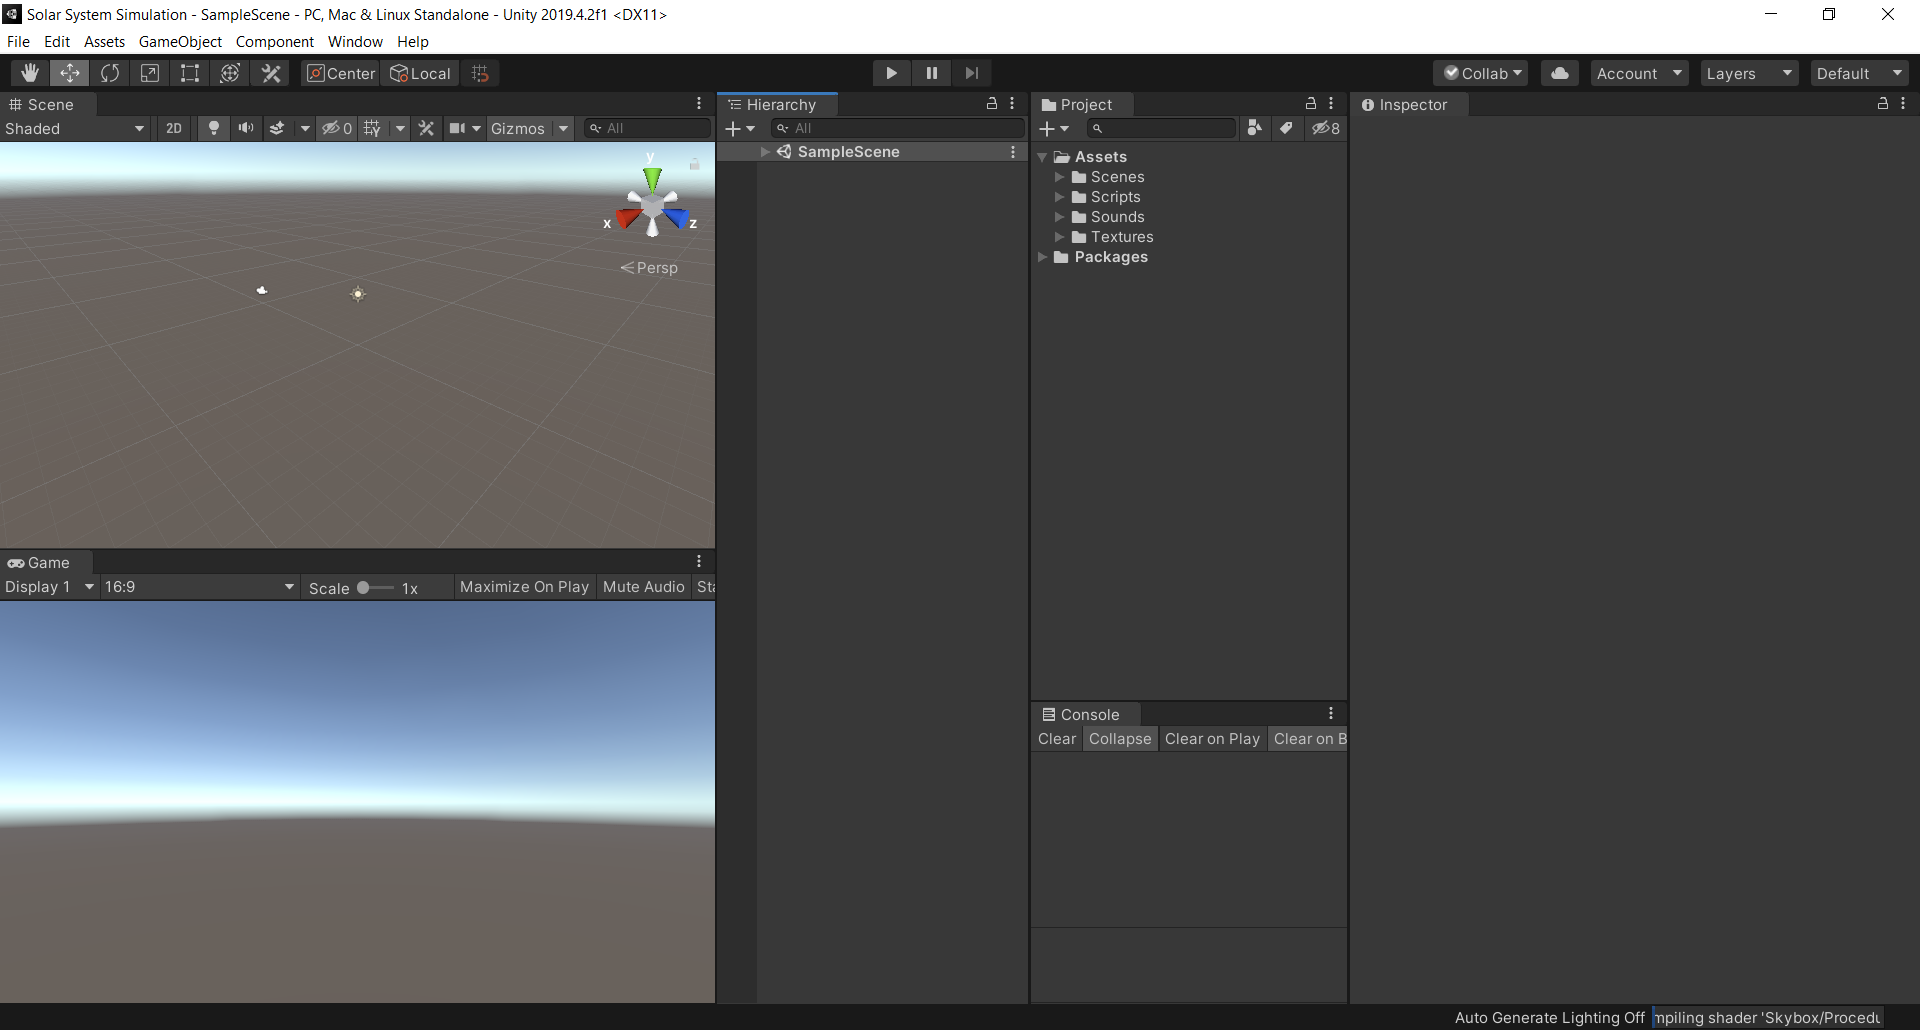
\includegraphics[width=\textwidth]{solarsystem_startscreen.png}\end{center}
We will be dealing with various game objects in a 3D cartesian system (pro-tip: to remember which axis is which colour, \textbf{RGB=XYZ}).
\subsection{Game objects and the transform component}

Now that we have a basic scene to work with, let's start out by adding the Sun, Earth and Moon as the first game objects. To do so, you might want to follow these steps (or maybe try to explore yourself how to do it):
\begin{enumerate}
	\item Click on the `GameObject' tab $>$ 3D Object $>$ Sphere
	\item In the `Inspector' panel, change the name of the object to `Sun'
	\item In the `Inspector' panel, adjust the position and scale parameters of the transform component
	\item Add the other 2 spheres, change their name, position and scale to suit them
\end{enumerate}
(If your game object initially appears in a weird position on your scene view, you can reset its transform by going to the `Inspector' panel $>$ right-click `Transform' $>$ Reset)
\vspace{6pt}

If you followed along these lines, you should have a screen that looks somewhat like this (could look slightly different based on the transform values you set):
\begin{center}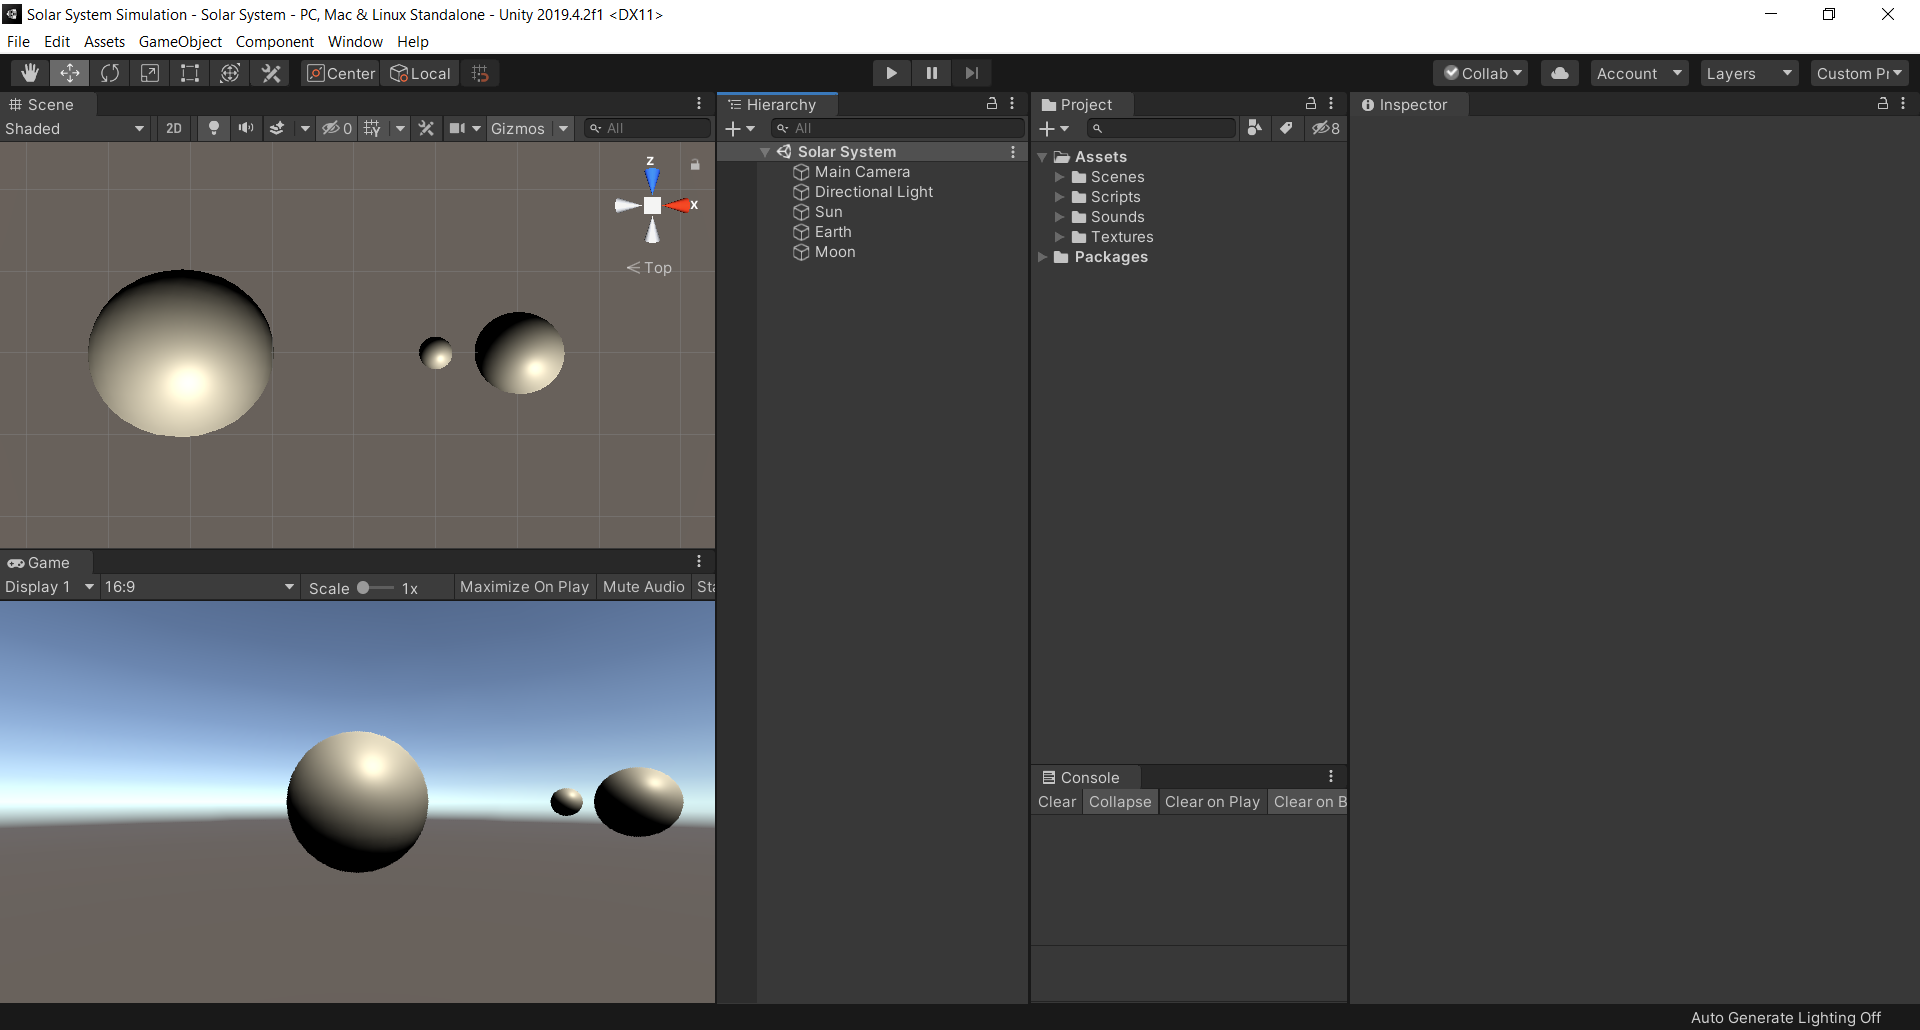
\includegraphics[width=\textwidth]{add_sun_earth_moon.png}\end{center}
As you can see, our objects have successfully been created in the `Hierarchy' panel and our scene and game views have been updated (Note: I have changed the position values in the transform component of the `Main Camera' object to focus the game view, however this is up to you).
\subsection{Adding behaviour to game objects}
Up till now, we have added the Sun, Earth and Moon as game objects. However, go into play mode and you will observe that they do not move. It is time to get them to rotate around each other appropriately. 
\vspace{6pt}

We do this by `adding behaviour' to our game objects. We do this through the use of scripts, which are nothing but files that contain code. This code tells Unity exactly how to get the game objects to behave with each other. Traditionally we would do this by writing the code ourselves, but as of now we have ready-made programs in the `Scripts' folder. From the names of the scripts, you might be able to (correctly) guess that we need to use the \texttt{RotateAround.cs} script here.
\subsubsection{Adding scripts}
Let us add the script to the Sun, Earth and Moon. Again there are multiple methods to add the script:
\begin{itemize}
	\item Click on the object in the hierarchy panel $>$ Click on `Add Component' in the inspector panel $>$ Click on `Scripts' $>$ \texttt{RotateAround.cs}
	\item Click \texttt{RotateAround.cs} in the projects panel $>$ drag and drop it on the desired game object
\end{itemize}
You will notice that a new `Rotate Around' component has been added into the inspector panel for the particular game object. It also contains two parameters - target (the object around which the selected game object will rotate) and speed (angular speed of rotation in degrees per second).
\vspace{6pt}

Note that the Earth rotates around itself as well as the Sun. This means we need to add the same script twice (similarly for the Moon as well).

\subsubsection{Adjusting script parameters}
Merely adding the script usually won't do anything. It is simply a component, and updating its parameter(s) is what will actually define the behaviour. I will elaborate the process for the `Earth' object, since there are 2 scripts we have to deal with:
\begin{enumerate}
	\item Target: drag and drop the `Sun' object onto target parameter of the first script in the inspector panel
	\item Speed: type in a suitable speed and test it in your game view and make further edits if any
	\item Similarly set up the second script by setting the target to the `Earth' object this time
\end{enumerate}
\begin{center}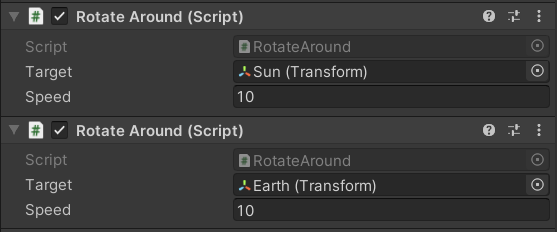
\includegraphics{rotatearound_earth.png}\end{center}
Complete these steps for the Sun and Moon as well (the Sun will need only one script, since it only rotates around itself), and please do not go into play mode yet. Note that there will not be any apparent effect of the objects rotating around themselves, but this is because we haven't added textures to them yet.
\subsubsection{Parent-child relationships}
Did you complete the above steps for the moon? Now go into play mode - I'm guessing you're having a pretty weird experience now. You're probably seeing the Moon chase the Earth and the distance between them increase. The reason for this delves a little bit into Mathematics and Physics, but I will discuss it in brief:
\begin{itemize}
	\item the \texttt{RotateAround.cs} script instructs the Moon to rotate around the `instantaneous center' of the Earth at any given point in time
	\item since the Earth is itself rotating around the Sun, the `instantaneous center' of the Earth is changing with time in the frame of reference of the scene view and so is the distance between the centers of the Earth and the Moon
	\item however, if we look from the frame of reference of the Earth (i.e. try to imagine that you're inside the Earth and at its center), what do you see? You will see apparently the Sun rotate around you, and the center of the Earth will appear stationary for you
\end{itemize}
If you still feel lost or get it partially, don't worry. You can look up the concept of `instantaneous center of rotation' on the internet and refer to some pretty good articles for more knowledge. 
\vspace{6pt}

Let's get back on track now. To fix this, we need to attach the Moon to the frame of reference to the Earth. In Unity language, we have to make the Moon a `child' of the Earth - this will make any motion of the Moon relative to the frame of the reference of the Earth. To do this, we simply click on the Moon in the hierarchy view and drag \& drop it onto the Earth.
\vspace{6pt}

Note that on setting the Moon as a child of the Earth, the transform components also change since the coordinates are now relative to the center of the Earth.
\subsection{Adding materials, lighting and audio}
We have set up the basic rotation scripts, but it is still just a couple of spheres rotating around each other. We can enhance the look of our solar system by:
\begin{itemize}
	\item making the Sun, Earth and Moon actually look like their solar system counterparts through the use of textures and materials
	\item removing the directional light \& adding a suitable background and lighting to the Sun
	\item adding basic audio to the simulation
\end{itemize}
\subsubsection{Adding materials}
A game object is made up of a 3D model. It can be thought of as a wire frame, and its material as the skin which wraps around this framework. Let us get into some theory about materials before we actually apply them to our solar system:
\begin{itemize}
	\item Material: all visible game objects have a material - however, it is only a set of parameters that specifies how the object should respond to light (it does not actually define the look of the object)
	\item Shader: this is the formula that takes the above parameters (position of individual triangles, relative position of light, material color values for each triangle) and defines the look of the object
	\item the shader has properties for texture maps (like emission, albedo, occlusion, etc), which in turn is the property of a material
\end{itemize}
If you're still confused, head over to this link to learn more about materials and shaders: 

\texttt{\href{https://gamedev.stackexchange.com/questions/45842/difference-between-material-and-shader}{https://gamedev.stackexchange.com/questions/45842/difference-between-material-and-shader}}
\vspace{6pt}

With the theory covered up, it is now time to actually add materials to our game objects:
\begin{enumerate}
	\item Go into the `Project' panel $>$ Assets $>$ Textures
	\item Drag and drop the `sunmap' texture on the Sun in the hierarchy view
	\item Notice how Unity automatically created a new `Materials' folder under the assets category - for organizational purposes rename the material to `Sun material'
	\item Repeat the process for the Earth and Moon
\end{enumerate}
Note that over here, we have only changed one property of the shader for each material. The texture map is what makes these objects look like entities in the solar system. By the end of this section, your window should look similar to this:
\begin{center}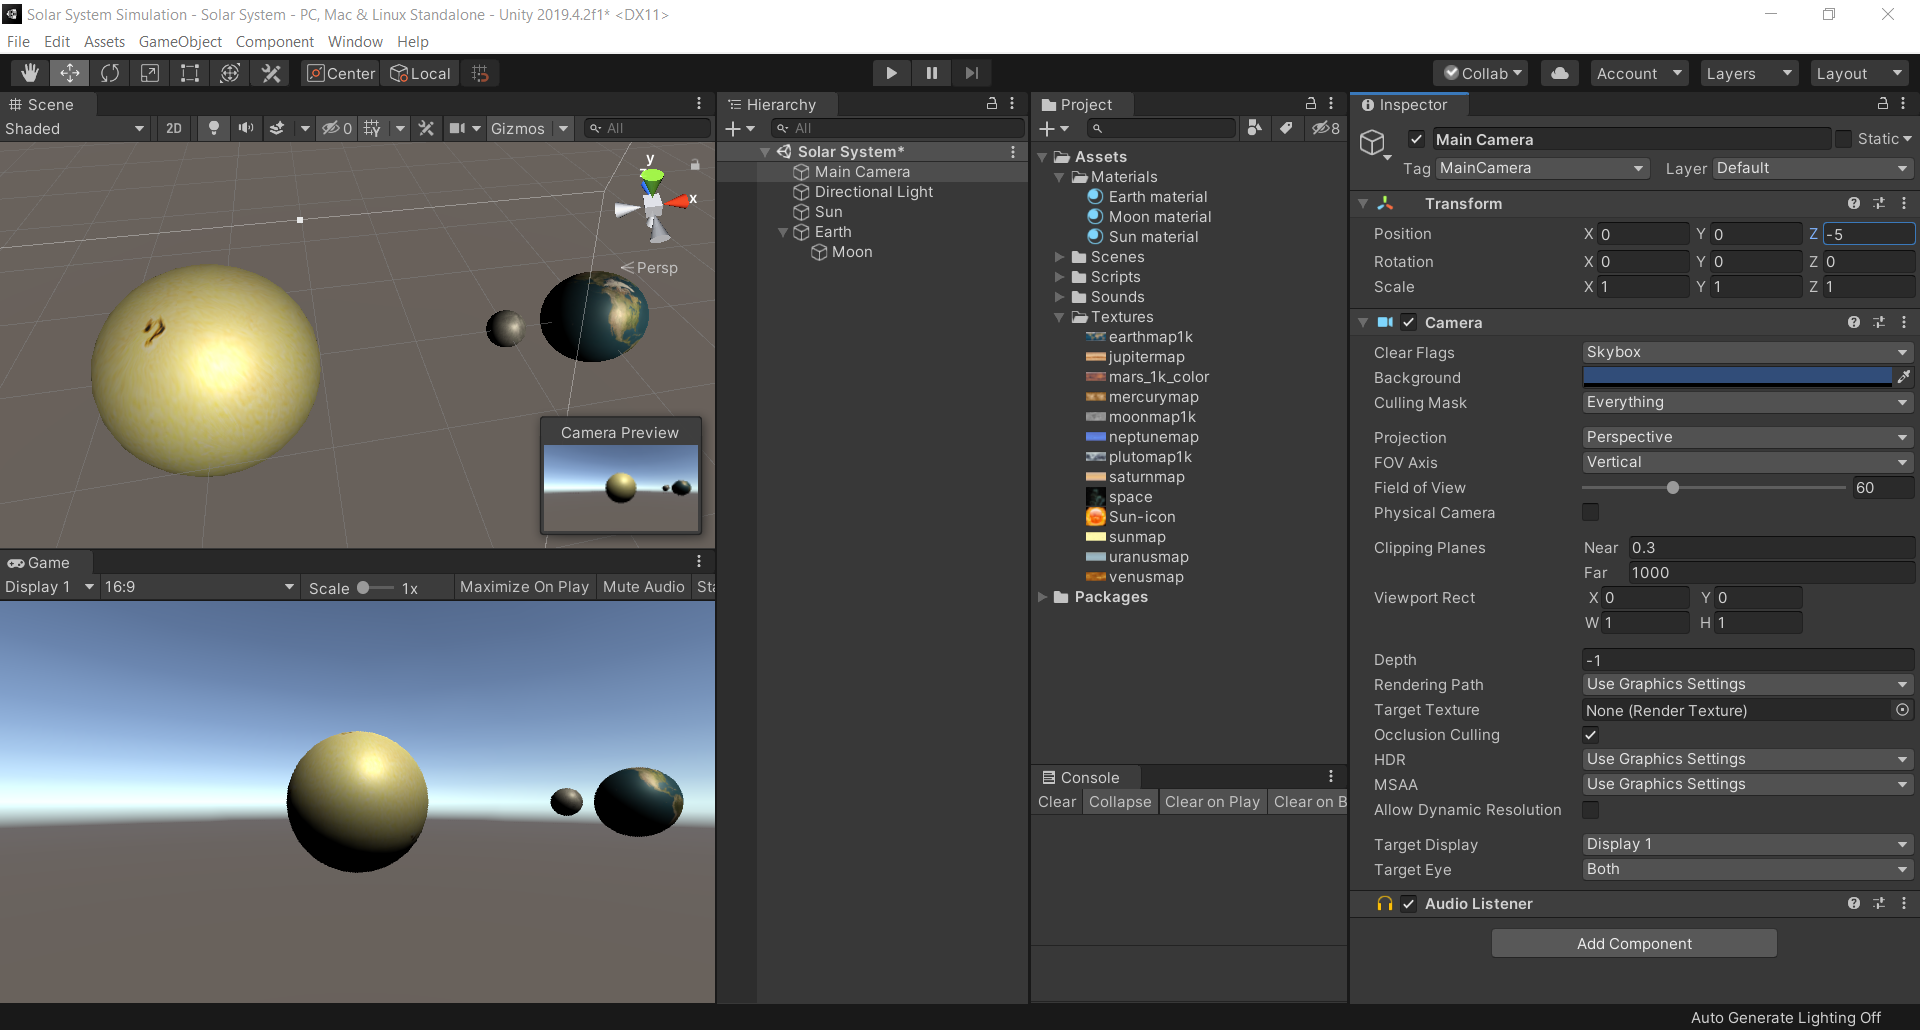
\includegraphics[width=\textwidth]{addng_materials.png}\end{center}
\subsubsection{Adding lighting}
We have 2 major lighting issues in this project - the Sun is not emitting any light of its own and the background doesn't look like space. Let us start by fixing the lighting for the Sun:
\begin{enumerate}
	\item Remove the `Directional Light' component from the hierarchy view (right-click $>$ Delete)
	\item Browse to `Sun material' in the projects panel and check the `Emission' property box
	\item It is possible to set a texture map for the emission color (which will essentially form a layer over the existing texture) - Go to the `Color' parameter under `Emission' $>$ Click the little dot next to `Color' $>$ Select a suitable texture map
	\item Set a suitable emission color (anything between yellow and orange should work for the Sun)
	\item (Optional, since 2019+ releases do not have this feature) Set the emission color brightness to an value to your liking
\end{enumerate}
\begin{center}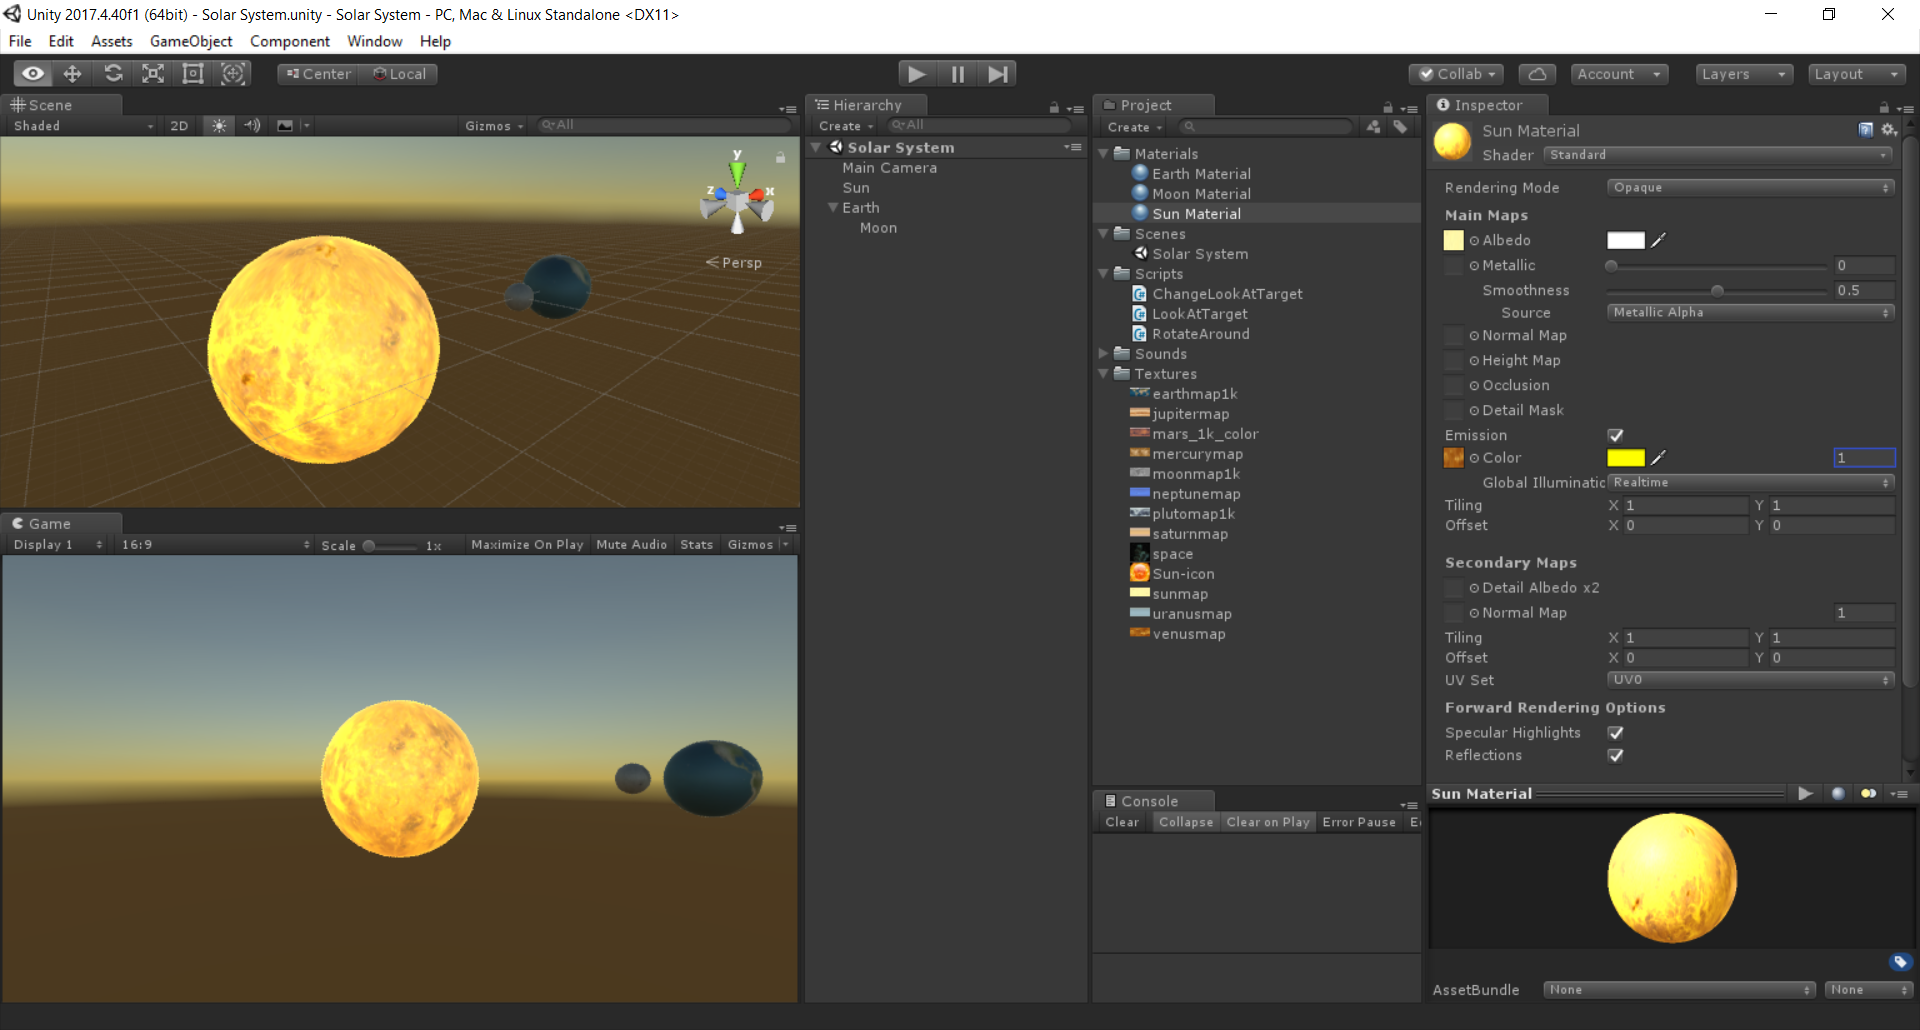
\includegraphics[width=\textwidth]{sun_emission.png}\end{center}
Now the sun has a little emission characteristic, but it still does not emit its own light onto the Earth and Moon. To do this, let us first understand the basic types of light objects in Unity:
\begin{itemize}
	\item ambient light: used for basic illumination (will be discussed later)
	\item directional light: used for illumination and establish the time of day if required
	\item point light: sends out light in all directions
	\item spot light: acts like the lights on a stage; illuminates a particular region
\end{itemize}
You will probably have guessed by now that we need to add a point light object as a child of the Sun. To do this, go to the `GameObject' tab $>$ Light $>$ Point Light. Reset its transform component if needed and set it as a child of the Sun. Play around with the parameters a little to get an appropriate lighting effect. You might want to rename this to something like `Sunlight'. 
\vspace{6pt}

If you have followed until now, your window should look similar to this (notice the difference in lighting between the 2 screenshots on this page):
\begin{center}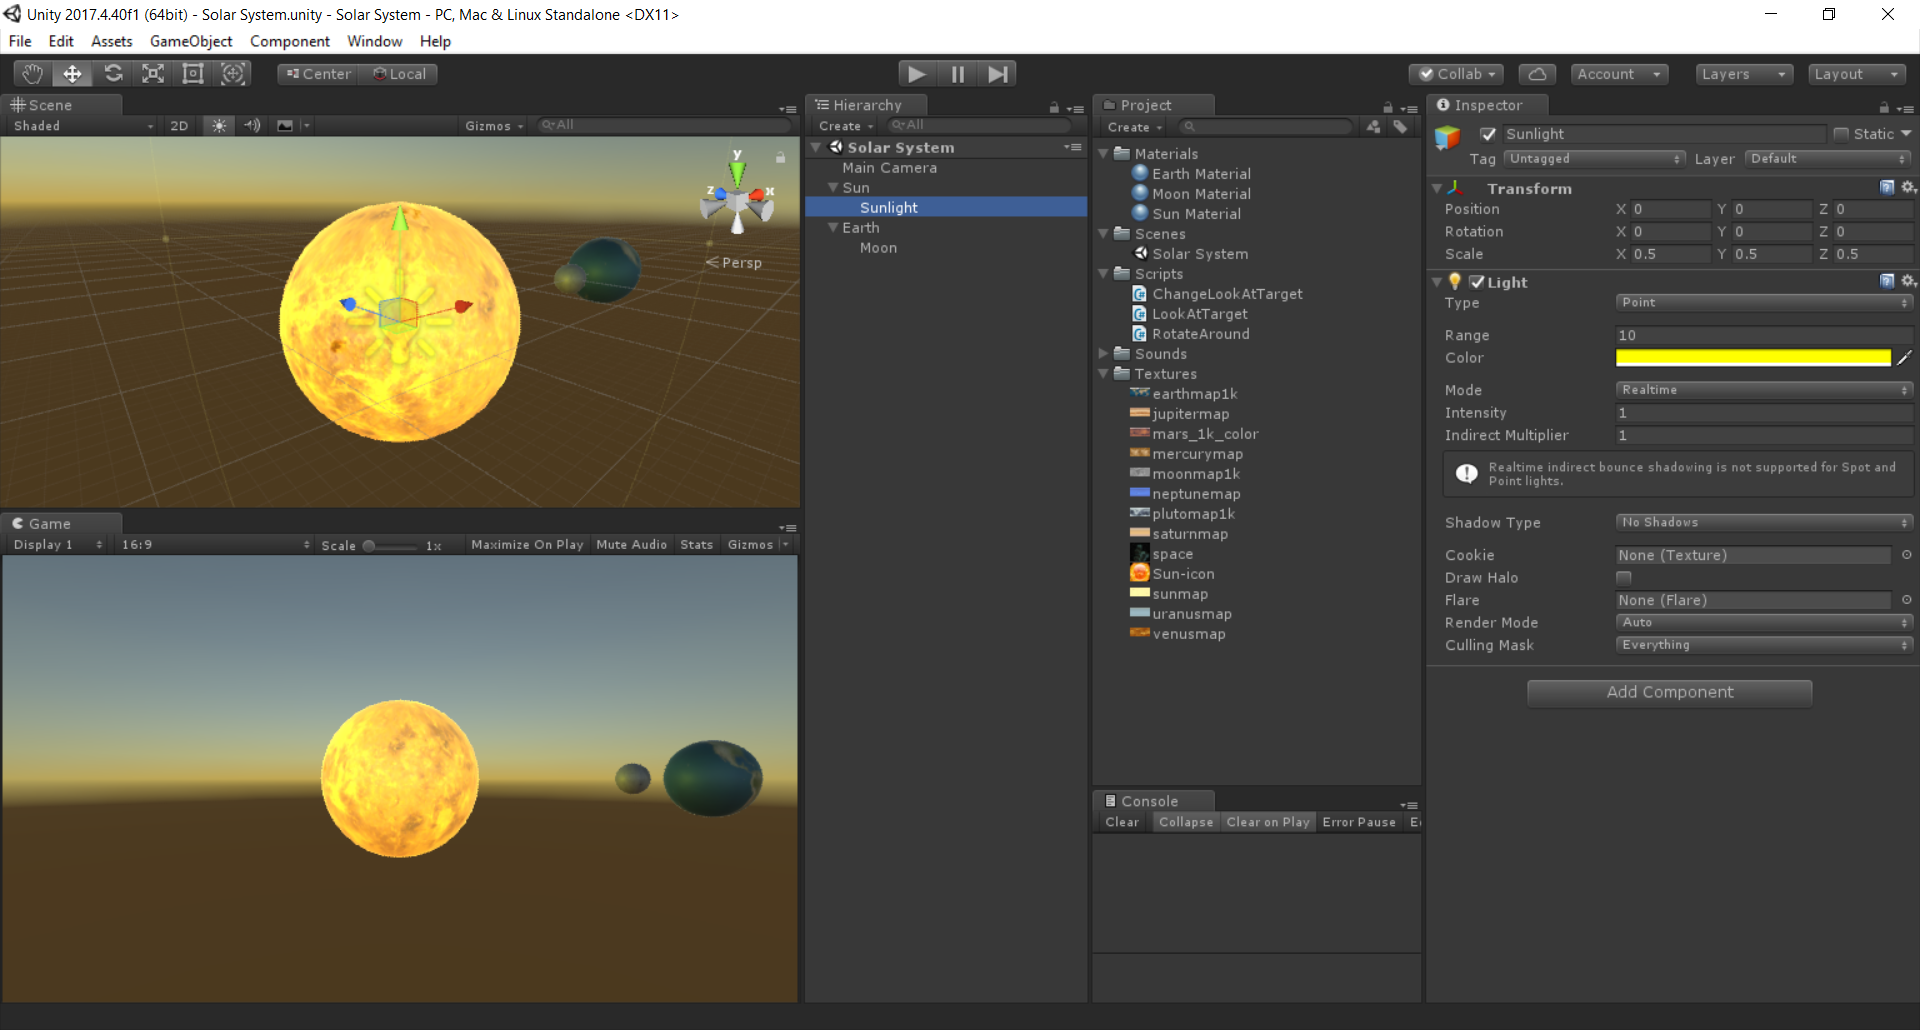
\includegraphics[width=\textwidth]{add_sunlight.png}\end{center}
Now that we have set up the lighting of the Sun, the only thing left to do is change the background and add ambient light. In Unity, the background is referred to as the Skybox. To setup the Skybox material:
\begin{enumerate}
	\item Go to the `Project' panel $>$ Click on `Create' $>$ Material
	\item Rename it to something appropriate
	\item In the `Inspector' panel $>$ Click the shader dropdown $>$ Skybox $>$ 6 Sided
	\item Set all 6 texture maps to the `space' texture (you could have multiple space textures and set them accordingly, but here we have only one to work with)
\end{enumerate}
Now it is time to add this material to the Skybox. To do this, go to the `Window' tab $>$ Lighting $>$ Settings (In some versions of Unity, you will have to go to `Window' $>$ Rendering $>$ Lighting Settings). Drag and drop the skybox material onto the corresponding property in the pop-up window.
\vspace{6pt}

We don't really need to add any ambient light, but we can do it by playing around with the parameters within the `Enviromment Lighting' section of the same window to add a little more flair to the scene. Once we are done with this, our scene should start looking a lot more like the solar system.
\begin{center}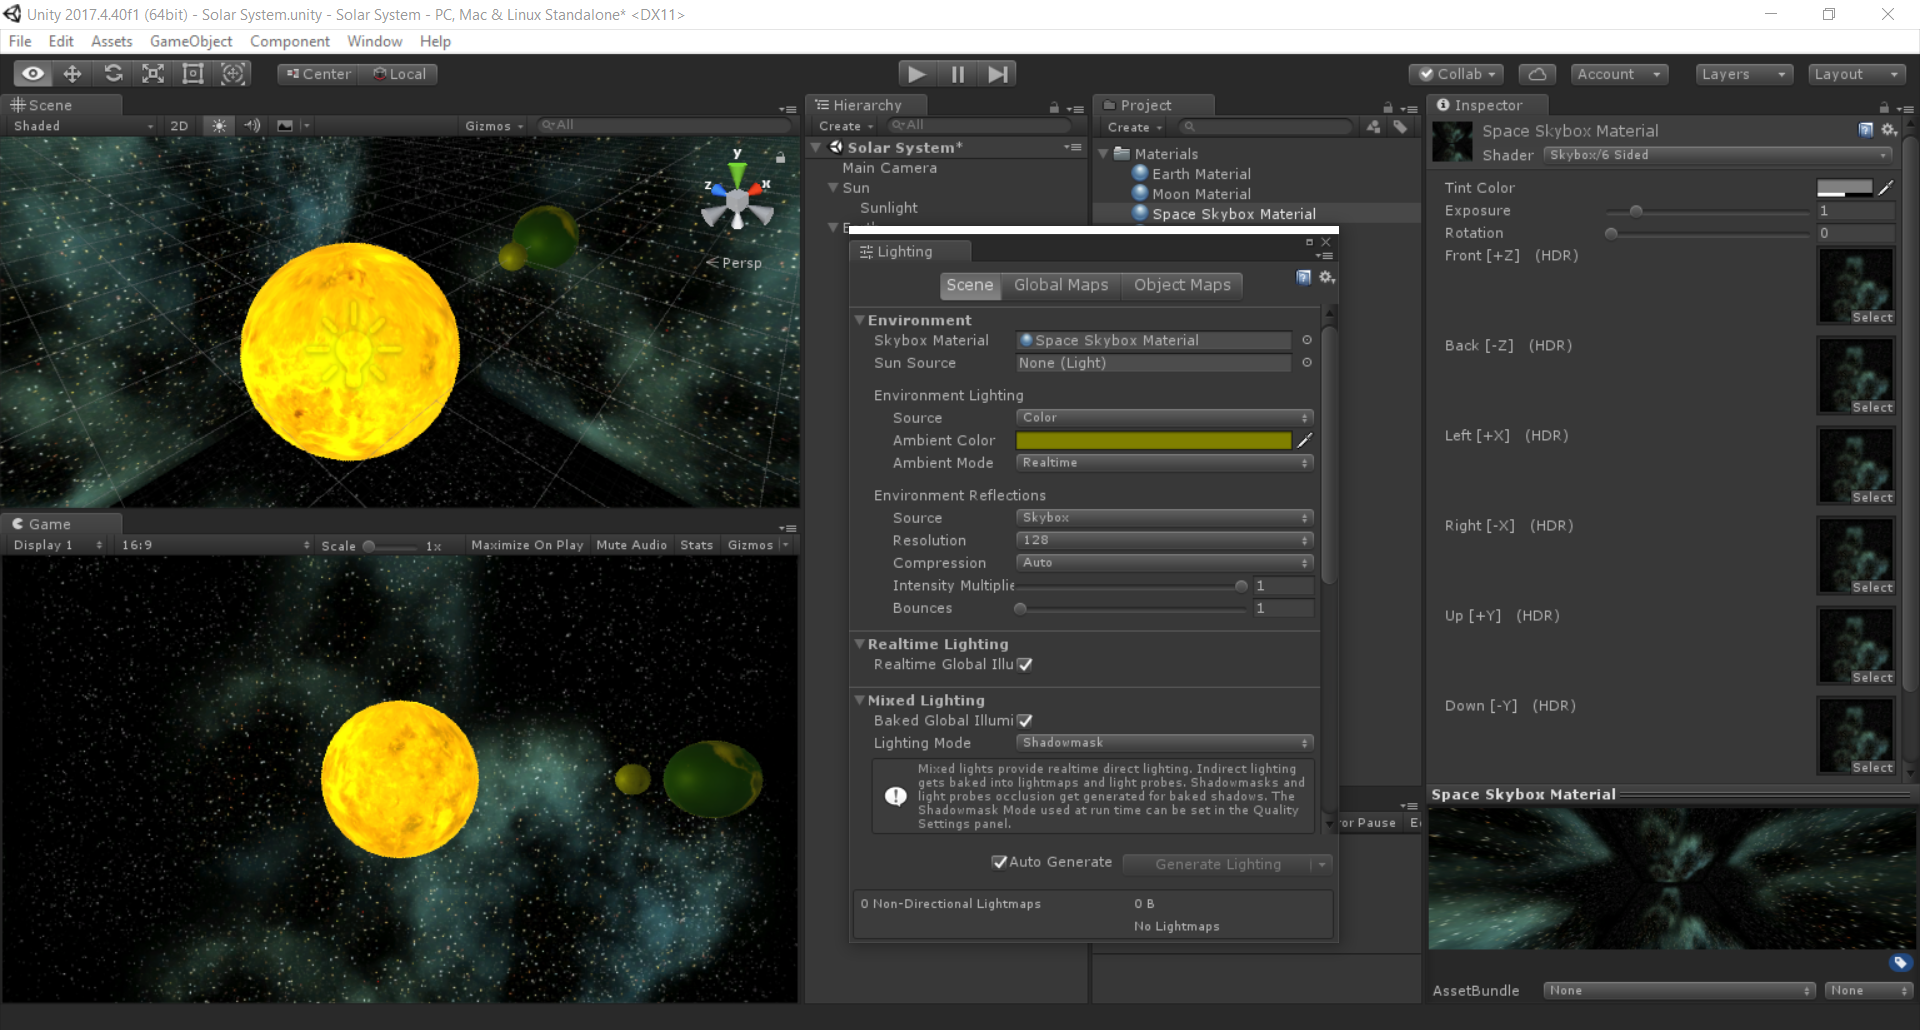
\includegraphics[width=\textwidth]{final_lighting.png}\end{center}
\textbf{NOTE:} While adding a lot of lights into a scene might make it look somewhat better, it is important to understand that more lights make the game more processor intensive and can adversely affect frame rates. It is hence advisable to work with as little light objects as possible.
\subsubsection{Adding audio}
While a solar system simulation doesn't necessarily need any audio, many other projects do. We will add some basic audio to illustrate some basic audio concepts in Unity. We might want to add a burning sound effect to the Sun and some sort of humming sound to the Earth which fades in and out as the distance of the Earth from the camera changes.
\vspace{6pt}

There are 2 audio components that we will work with. The audio source component has to be attached to the game object which is meant to emit sound, while the audio listener is often attached to a camera object. As the name suggests, the audio listener picks up the sound emitted from the audio sources (intensity depends on the distance between the source and listener). The listener is a simple component -  it has no properties and can only be turned on or off.
\vspace{6pt}

To add the audio source component to the game objects, follow these steps (I will illustrate it for the Earth object, since we will also need to edit 3D sound settings for it):
\begin{enumerate}
	\item In the `Inspector' panel $>$ Add Component $>$ Audio $>$ Audio Source
	\item From the project panel, drag and drop the `dronehum.aif' audio file onto the AudioClip parameter in the inspector panel (if you go into play mode, you will hardly notice the fading effect of the sound)
	\item To make the fade effect more prominent, go to the Audio Source component $>$ 3D Sound Settings $>$ set the Min and Max distances to appropriate values and adjust the volume rolloff to your liking
\end{enumerate}
Repeat the same process for the Sun (since it is at a fixed position, no need to change any 3D sound settings. If you followed along, your audio source component settings should look similar to this:
\begin{center}
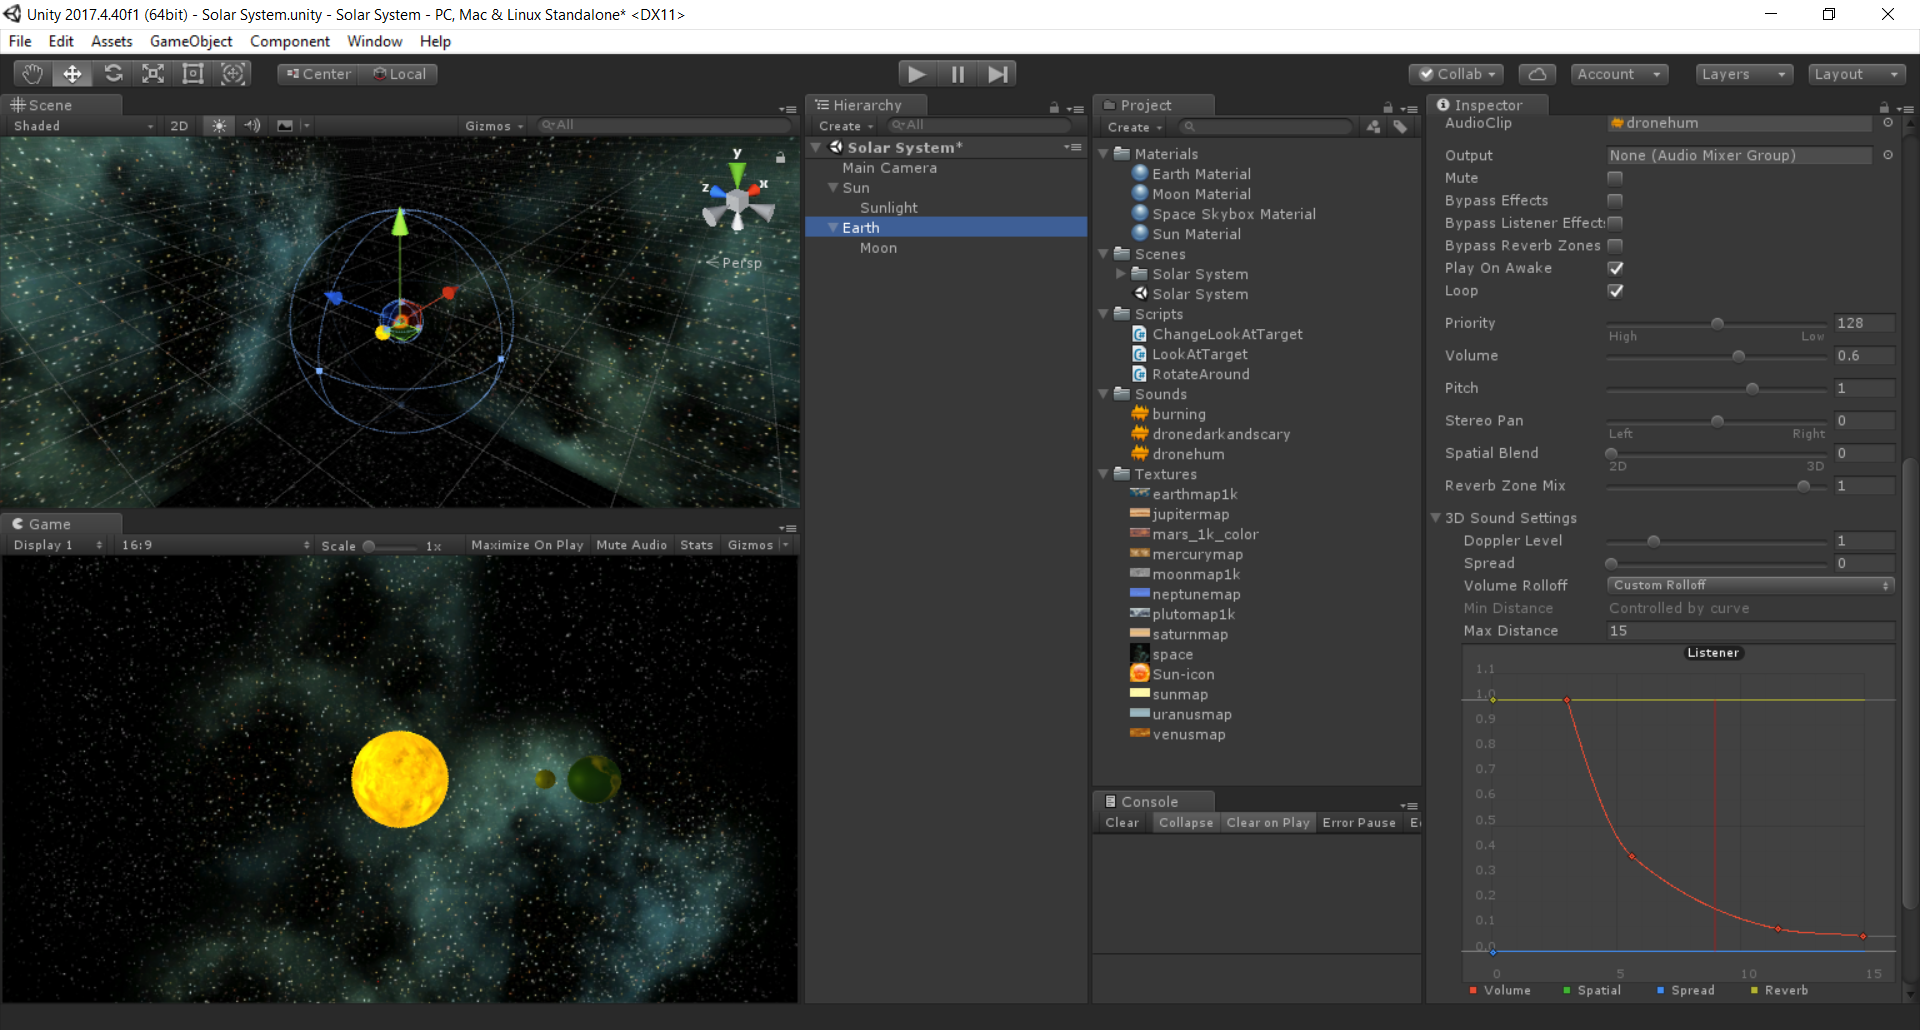
\includegraphics[width=\textwidth]{adding_audio.png}
\end{center}
\subsection{Adding cameras and adjusting views}
A camera object in Unity is far from its real life counterpart. What a camera in Unity essentially does is project the 3D geometric information onto a 2D screen. We can choose to have multiple cameras in a single scene and show them simultaneously on screen.
\vspace{6pt}

There are 2 types of 3D projections - perspective and orthographic. The perspective projection is what we have in our camera now, since the Earth appears bigger as it moves closer and vice-versa - it renders everything within its `view frustum'. Orthographic projections can probably be found in case of top-down or isometric views - the camera maintains the same scale of the object irrespective of the distance (a good example of this is \textit{SimCity}).
\begin{center}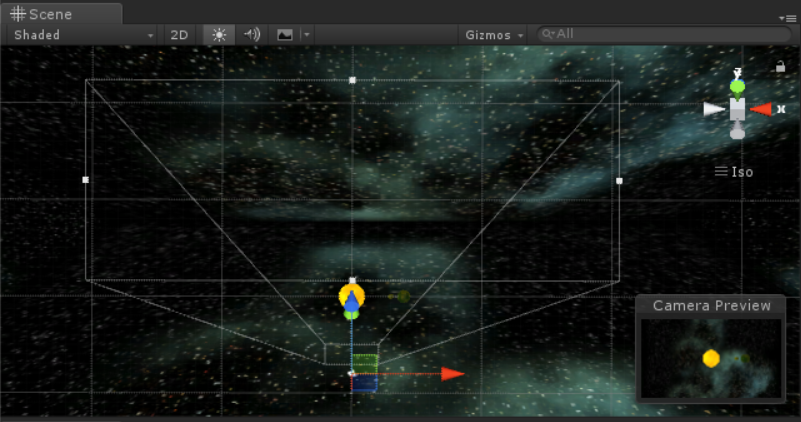
\includegraphics{view_frustum.png}\end{center}
The view frustum is better described by the above image. The white outlines determine the field of view and the near and far clipping planes (set right now at 2 and 20 metres respectively). If, for instance, the Earth were to come within 2m distance or go farther than 20m distance from the camera, the object would not be rendered.
\vspace{6pt}

For the purpose of applying these camera concepts, we will create a second camera to show a top-down view of our solar system and position it in a little `mini-window'. To add and position the camera suitably, follow these steps:
\begin{enumerate}
	\item Go to the `Hierarchy' panel $>$ Create $>$ Camera (the game view will suddenly change, since Unity reads this as the new active camera)
	\item Reset its transform if needed and rename it to something suitable
	\item Position and angle the camera so that it provides a top-down view of our solar system model
	\item Go to the `Camera' component in the inspector $>$ Projection $>$ Orthographic
	\item Play around with further properties till you get a view that you like
\end{enumerate}
So we have added our second camera. However the game view shows only the view from this new camera object. Since this is going to be positioned in a `mini-window', we probably need to update some further settings within the inspector. Follow these steps to set up the minimap camera window:
\begin{enumerate}
	\item In the `Inspector' panel $>$ Camera $>$ Viewport Rect (this is basically a set of origin coordinates size of the rectangle on the screen to which the camera outputs)
	\item Set suitable values for width and height (width of 0.25 means that the rectangle will have one-fourth the width of the screen)
	\item (Optional) To make the background color of the minimap different, in the same component $>$ Clear Flags $>$ Solid Color (set any color you like)
\end{enumerate}
Note how the main camera view appeared again. By now you should have a screen looking like this:
\begin{center}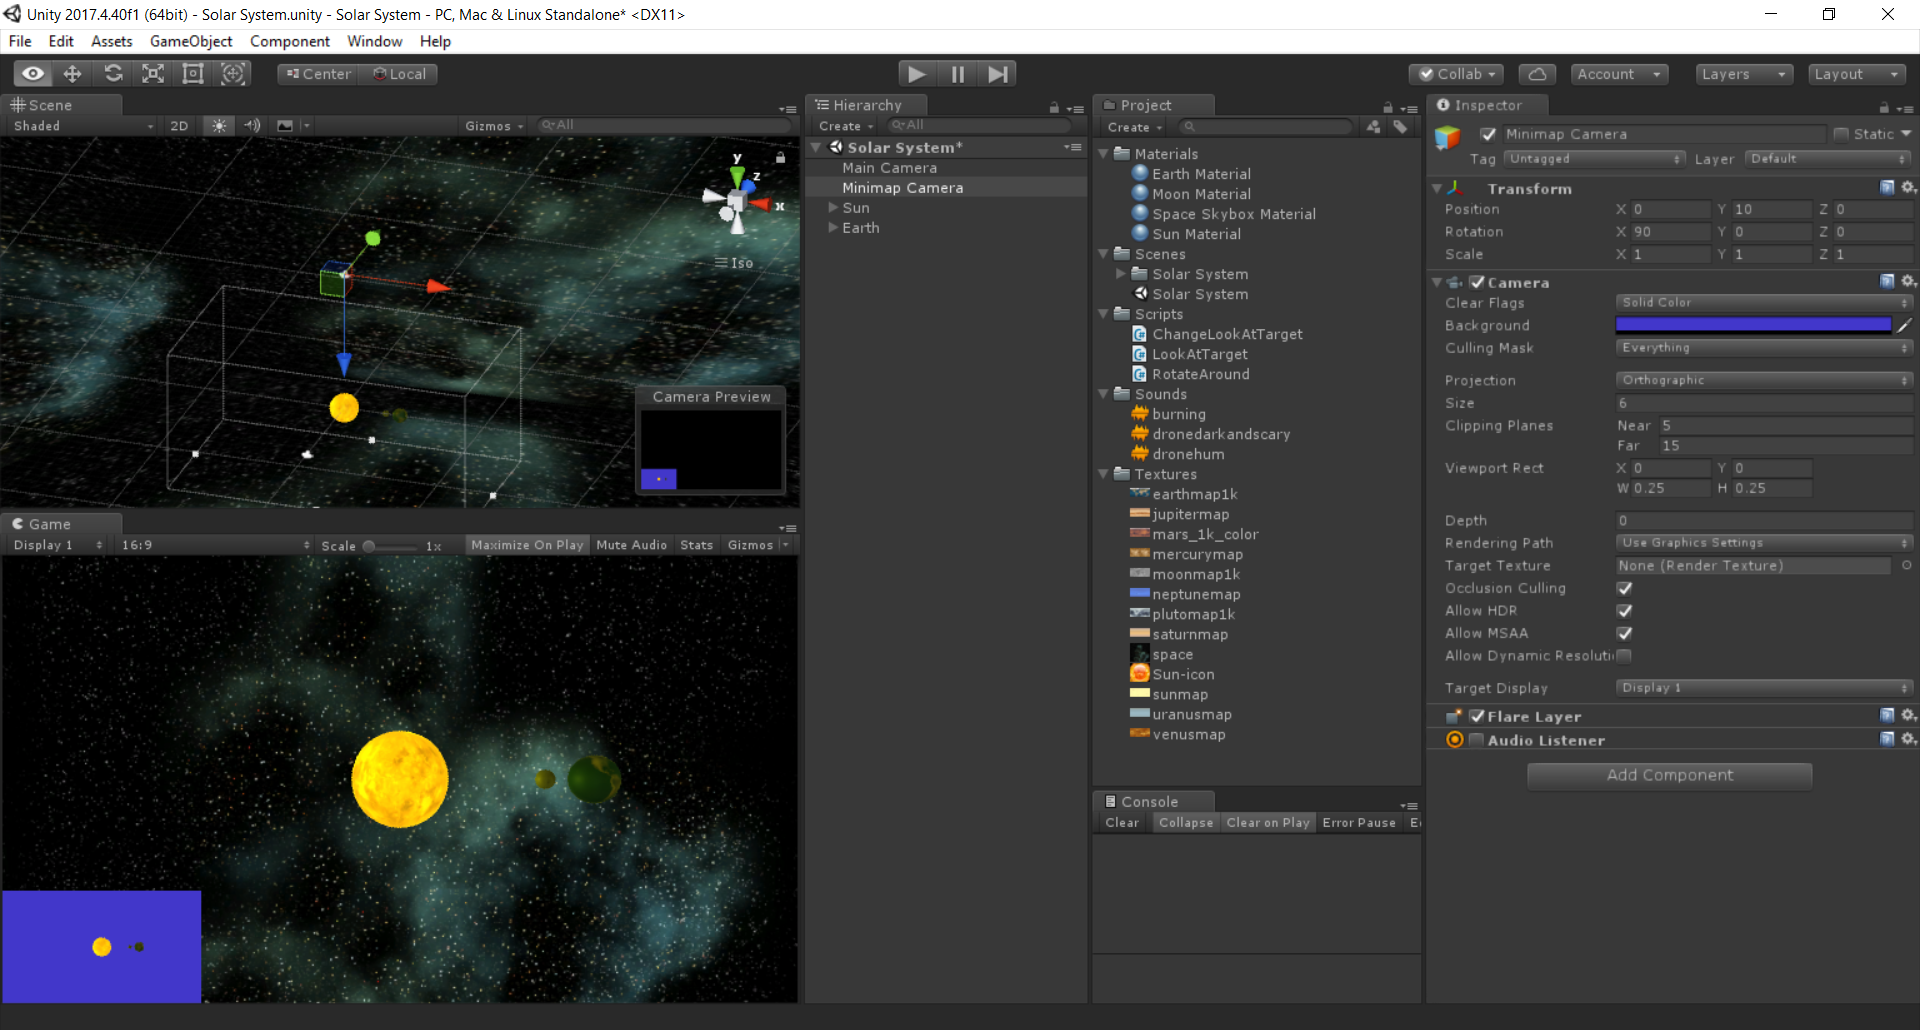
\includegraphics[width=\textwidth]{minimap_camera.png}\end{center}
\vspace{6pt}

\textbf{NOTE:} We now have 2 camera objects and hence 2 audio listeners. It is highly advised to have only one audio listener component switched on at any given point of time - otherwise Unity will pick one of those two, which may not be the one we want. To avoid this, switch off the audio listener component on the second camera (or remove it altogether since we won't be using it anyway).

\subsection{Finishing, building and deploying a project}
We have essentially completed our simulation of the solar system. We could do some more finish work like (this is all essentially based on the concepts covered earlier so I will not discuss this in detail):
\begin{itemize}
	\item add other planetary bodies  to complete the solar system
	\item figure out how the \texttt{LookAtTarget.cs} and \texttt{ChangeLookAtTarget.cs} scripts work (hint: they are meant to work together so that clicking on the Earth will focus the main camera on the Earth and so on)
\end{itemize}
Take some time out to test your final project to test for any bugs. It is highly unlikely that this project will have any, but it is still a good idea to do so. By the end you should have something that looks like this:
\begin{center}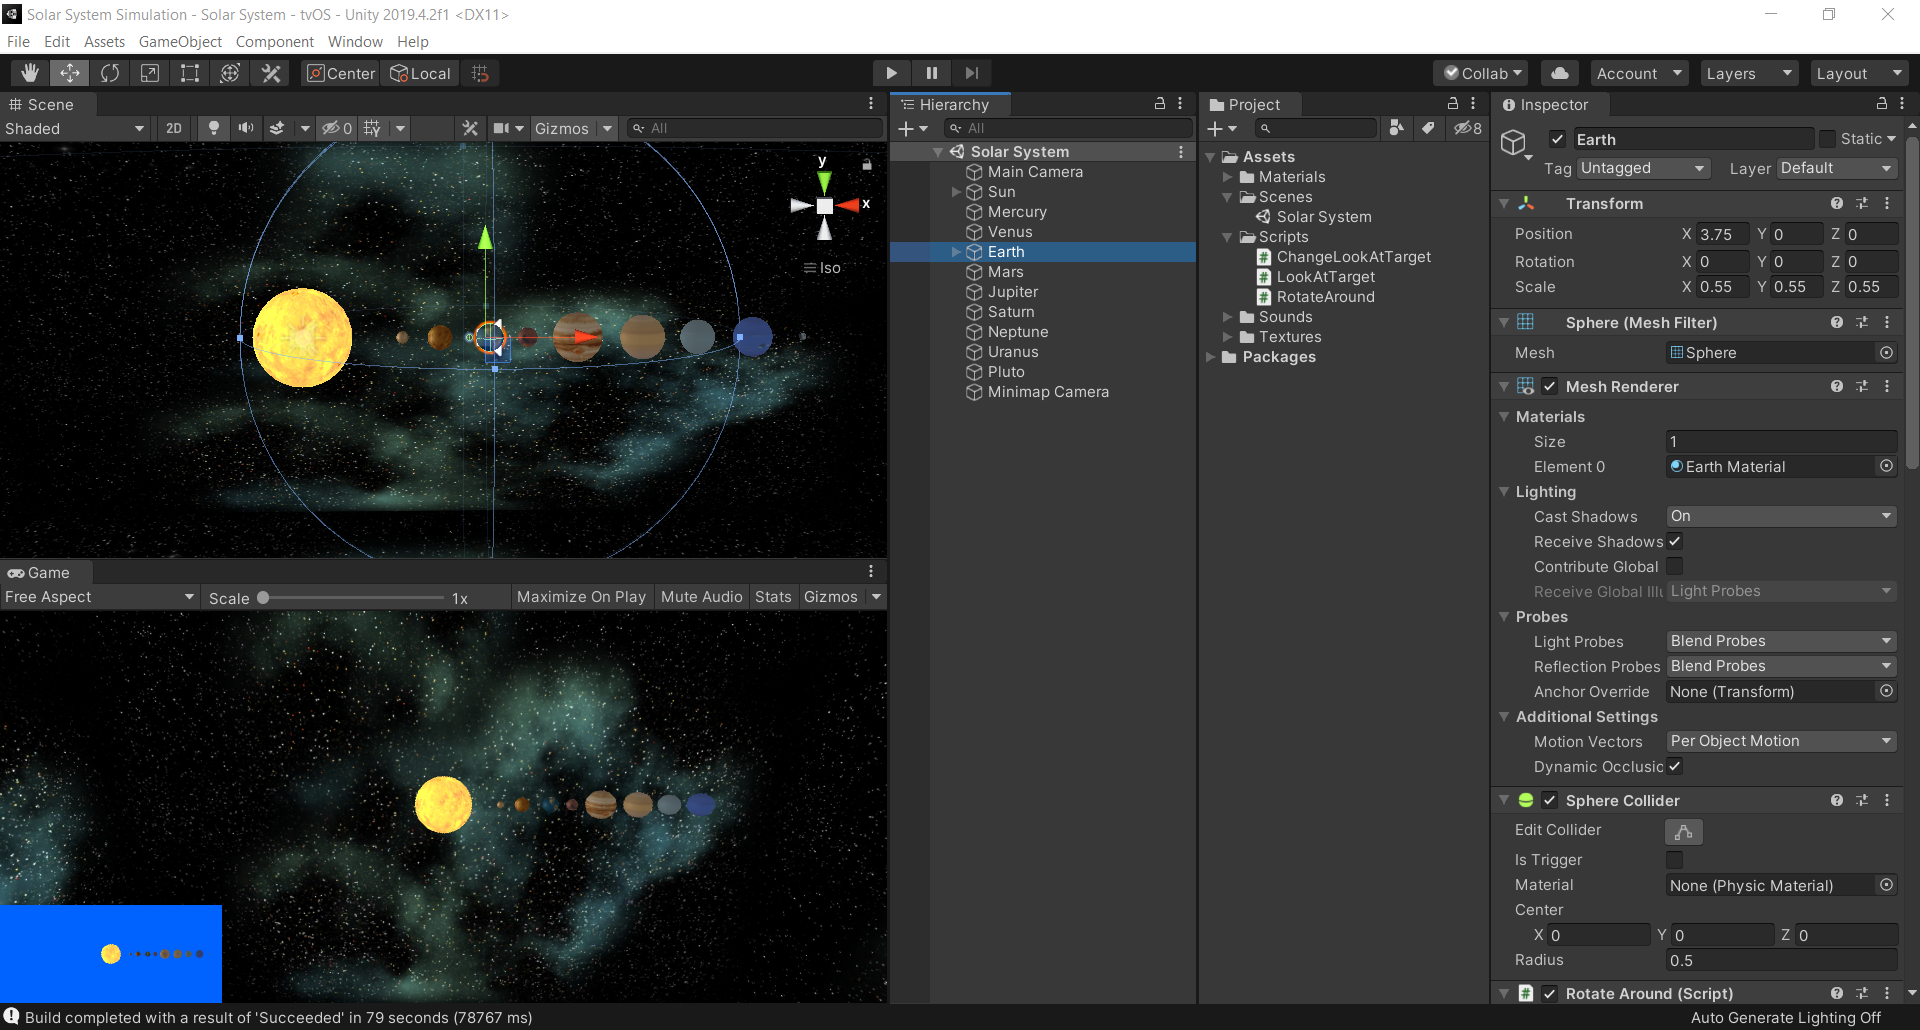
\includegraphics[width=\textwidth]{solarsystem_final.png}\end{center}
Once you're done testing, it is time to finally build it so that it can be launched as an application from any specific platform. This can be done in the following manner:
\begin{enumerate}
	\item File $>$ Build Settings
	\item Drag the `Solar System' scene from the projects panel into the `Build Settings' window
	\item Select the platform for which you want to build the application. If needed, click on `Switch Platform'
	\item Click on `Player Settings ...' and play around with the settings to your liking (do not mess around too much, the default settings work well for the most part)
	\item Click on `Build', select a destination and wait for the build to be complete
	\item Launch the application to see if it works successfully
\end{enumerate}
\textbf{NOTE:} Again for organizational purposes, it is better to save all your builds in the Unity project folder itself in a folder called `Builds' (eg: for a Windows build, save it in Builds $>$ Windows and so on).

\hrulefill
\begin{center}\textbf{END OF WEEK 2}\end{center}
This is the end of the documentation from Week 2 of the course. In the next project, will be creating an actual game called `Roller Madness' which will put into action all the previously discussed concepts and more. Continue reading forward, or head over into Unity and try out some stuff yourself.

\hrulefill
\pagebreak
\section{Roller Madness}
\textit{(This section is in the works along with notes from Week 4 as well. I will probably be finishing Week 4 first since I am already going through the Week 4 course material at this time. However, there shouldn't be any major loss if you do Week 4 before Week 3. Expect it to be up in about 2 weeks.)}

\hrulefill
%\begin{center}\textbf{END OF WEEK 3}\end{center}
%This is the end of the documentation from Week 3 of the course. In the next project, will be creating an actual game called `Box Shooter' which will put into action all the previously discussed concepts and more. Continue reading forward, or head over into Unity and try out some stuff yourself.

%\hrulefill
\pagebreak
\section{Box Shooter}
Up till now we have only used ready-made scripts. However it is important to be able to write our own code and modify existing code as well, irrespective of our role in the dev team. With a working knowledge of programming, we can go much further in Unity as well as other tools like Maya, Blender, etc. One must strive to gain at least an intermediate level of understanding in programming which will allow them to grasp the core language, write code and modify code from an example source.

\subsection{Unity programming concepts}
Unity follows an object-oriented approach to programming. Much like the real world, everything here is considered an object - it has properties (variable type, size, etc) and methods (functions which enable performing actions using code) associated with it. Most of the assets we have worked with up till now were visual objects. These objects have their properties (i.e. components) and methods (parameter values).
\vspace{6pt}

One important concept in object oriented programming is classes. Classes are templates for creating objects, much like prefabs which we used in the previous project. For example there could be a class for a 	`clock' object that defines how a general clock should function, but individual clocks generated from this class will have their own properties like color, timezone, etc.
\vspace{6pt}

Let us now discuss more about programming in Unity:
\begin{itemize}
	\item the language used to write code for Unity is C\#
	\item a C\# script can either be created from scratch by `Project' panel $>$ Create $>$ C\# Script, or be imported from an existing source and later modified
	\item a script is just another type of asset like sounds, textures, etc
	\item scripts can be attached as components to game objects in a scene
\end{itemize}
\begin{center}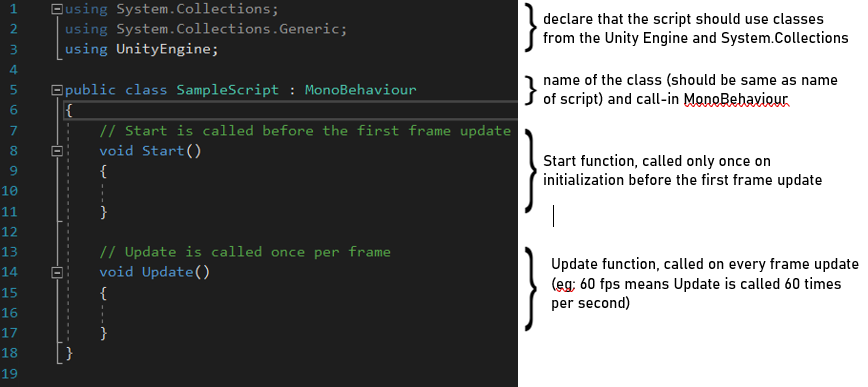
\includegraphics[width=\textwidth]{program_basic_structure.png}\end{center}
A typical script template generated by Unity is as above:
\begin{itemize}
	\item part 1: instructs the scripts to use classes from \texttt{UnityEngine} and \texttt{Systems.Collections} (these are namespaces which define various types of objects like lists, queues, arrays, etc)
	\item part 2: \texttt{public class} indicates that this class will be visible as a component in Unity (public classes \& variables are generally seen as components in Unity)
	\item part 2 (continued): \texttt{MonoBehaviour} is the base class from which every script in Unity derives (in essence, \texttt{SampleScript} is our custom class which uses stuff from the broader \texttt{MonoBehaviour} class) - Mono is an open-source implementation of Microsoft's .NET framework
	\item part 3: variables \& functions that make up the details of the \texttt{SampleScript} class
\end{itemize}
\pagebreak
Let us now look at a more complete C\# script:
\begin{center}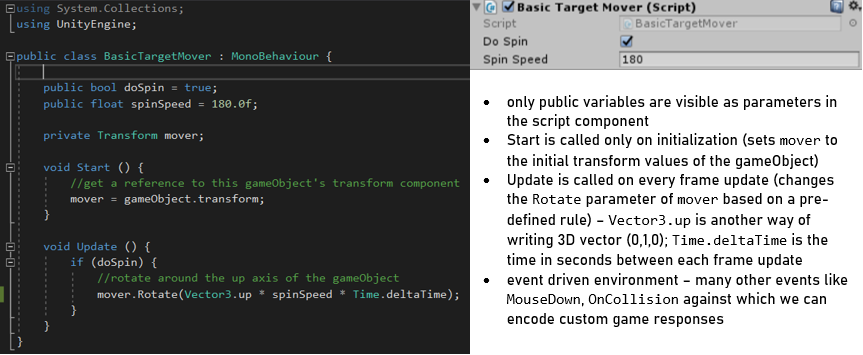
\includegraphics[width=\textwidth]{basic_target_mover.png}\end{center}
The event driven environment means that we will often be adding functions to the class(es) to respond to events that occur in certain stages of the game.
\begin{center}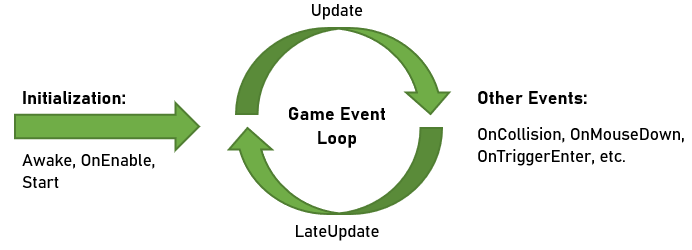
\includegraphics{ecent_cycle.png}\end{center}
Just like \texttt{Start}, we have 2 other events \texttt{Awake} and \texttt{OnEnable} which allow us to set things up before the first frame update occurs. After this, the game is set into an event loop (each loop usually lasting a frame) - the \texttt{Update} and \texttt{LateUpdate} functions provide a way to keep a check on things while the game is playing. Finally, there are certain specific events that the program can be instructed to respond to in a certain manner (eg: \texttt{OnMouseDown} causes the camera view to shift down).
\subsubsection{Referencing gameObjects in scripts}
When a script is attached to game object, it can be referred to as either \texttt{this.gameObject} or simply \texttt{gameObject}. The following is a simple program that causes the transform of the object to change: 
\begin{center}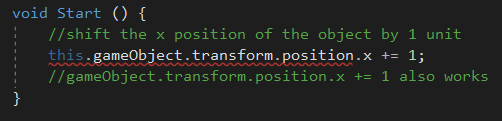
\includegraphics{reference_local_gameobject.png}\end{center}
For referencing any other game object that the script is not attached to, we need to define a public variable of type gameObject that we attach to another game object/prefab in the editor. They can further be searched in the editor either using object names or tags. The following is a program to change the transform of global game objects:
\begin{center}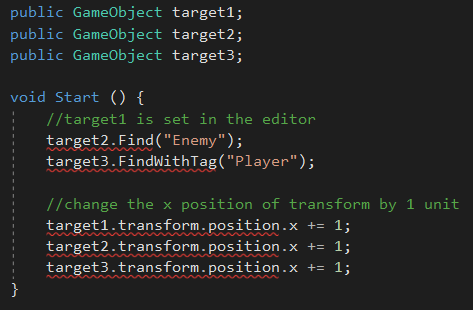
\includegraphics{reference_global_gameobject.png}\end{center}

\subsubsection{Referencing components in scripts}
Every property you see in the Unity Editor for a component can be reference and often modified through code. For example, in both of the above programs we referenced the position (\texttt{gameObject.transform.position.x}) along the X-axis and also modified it.
\vspace{6pt}

Quite often, there are multiple ways of implementing actions into code. Sometimes one is more efficient than the others. For example, \texttt{gameObject.transform.position.x += 1} and \texttt{gameObject.transform.Translate (1,0,0)} do exactly the same thing.
\vspace{6pt}

Not all components are properties of a game object like transform. To reference and/or manipulate these, we use the \texttt{gameObject.GetComponent<TYPE>()}
function. The following program illustrates the above concept to the `RigidBody' component:
\begin{center}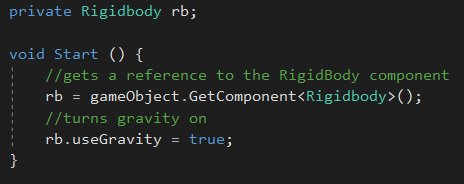
\includegraphics{reference_components.png}\end{center}
\textbf{NOTE:} Consider the following points while programming in Unity:
\begin{enumerate}
	\item The name of the class \textit{must} be the same as your script name. If you do change the name of your script, you will have to change the name of the class too - Unity does \textit{NOT} automatically do this
	\item If you find yourself stuck, Unity has an excellent documentation (\texttt{\href{https://docs.unity3d.com/}{https://docs.unity3d.com/}}) - this can also be accessed through many IDEs like MonoDevelop and VS Code (Help $>$ Unity API Reference)
	\item Use the community forum (\texttt{\href{https://unity.com/community}{https://unity.com/community}}) to your advantage - if you're stumbling upon an error, it is more than likely that someone else has too
	\item Finally, here is a quick reference sheet on writing basic C\# code: \texttt{\href{https://omprabhu31.github.io/gamedev/notes/gamedev_intro/scripting_reference_sheet.pdf}{Reference Sheet}}
\end{enumerate}
\subsection{Setting things up}
In this project, we will dive a lot deeper into Unity by building out a custom game using our own custom scripts. Most of the time in this project, we will be modifying existing code rather than making scripts from scratch. Some of the concepts we will cover are:
\begin{itemize}
	\item creating custom C\# scripts using an IDE and basic debugging techniques
	\item use of classes, variables and functions to respond to events
	\item instantiate prefabs dynamically, obtain user input and update user interface through code
\end{itemize}
Similar to earlier projects, if you are trying this out yourself, you will have to find the assets in the GitHub repository. Once you have them downloaded, import them into the project. Since this is a single unity package file, import it by going to `Assets' $>$ Import Package $>$ Custom Package... $>$ Browse to the local file location.

\subsection{Using scripts to move objects}
In this subsection, we will apply the concepts of public variables, floating point numbers, boolean values and referencing components to create a basic script for moving a target object. Firstly, create a 3D object (I have created a cube) and name is as `Target' and apply the Target-Positive Material to it.
\subsubsection{Basic object movement}
A script to induce basic movement in a game object might look like this:
\begin{itemize}
	\item \texttt{Vector3.up}: a representation of the 3D vector (0,1,0) - references the Y component of the rotate and position properties of the transform respectively
	\item \texttt{Time.deltaTime}: normalizes the motion for different frame rates
	\begin{itemize}
		\item[$-$] without this, the spinning would be slower on 15 FPS compared to 60 FPS
		\item[$-$] multiplies by the time in seconds between frames (i.e. for 60 FPS, 1/60)
		\item[$-$] for example at 60 FPS, Update is called 60 times per second - during every update, object rotates through (0,3,0) so total rotation in one second is (0,180,0)
		\item[$-$] in contrast for 15 FPS, Update is called 15 times per second - during every update, object rotates through (0,12,0) so total rotation per second is again (0,180,0)
		\item[$-$] as a result, consistence of spin motion is maintained but smoothness of the motion may vary	
	\end{itemize}
	\item \texttt{Mathf.Cos(Time.timeSinceLevelLoad)}: cumulative time since level load (converted to radians) - facilitates harmonic motion of the target object
\end{itemize}
\begin{center}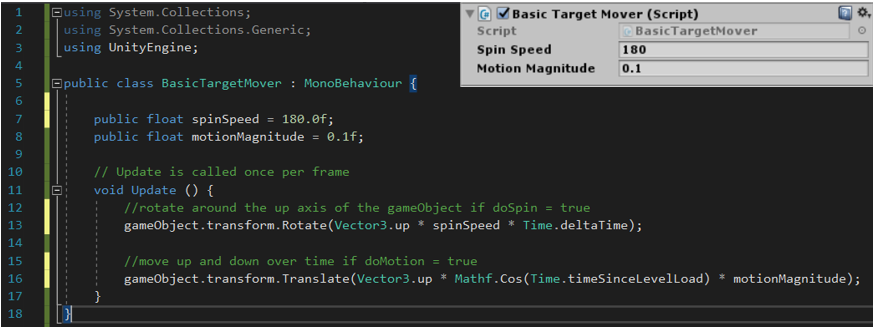
\includegraphics[width=\textwidth]{basic_target_mover_float.png}\end{center}
\subsubsection{\texttt{bool} datatype and \texttt{if} statements}
With the above code, we can make our target game object spin as well as move up and down. If we only want it to spin, we can set the Motion Magnitude value to 0 within the editor (this will not affect the value in our script), and similarly for only motion. While this is easy enough, it is not user-friendly and game designers might want simple options to switch these properties on and off. When faced with words like on and off, true and false, etc, a programmer's instinct leads them to work with the boolean datatype.
\vspace{6pt}

The bool datatype is a relatively simple one - it can store only values 0(false) and 1(true). We can define 2 bool variables named \texttt{doSpin} and \texttt{doMotion} and write if statements so that:
\begin{itemize}
	\item spin motion occurs only if \texttt{doSpin} is true
	\item vertical motion occurs only if \texttt{doMotion} is true
\end{itemize}
And of course, we can individually switch these on/off in the editor without affecting values in the script file.
\begin{center}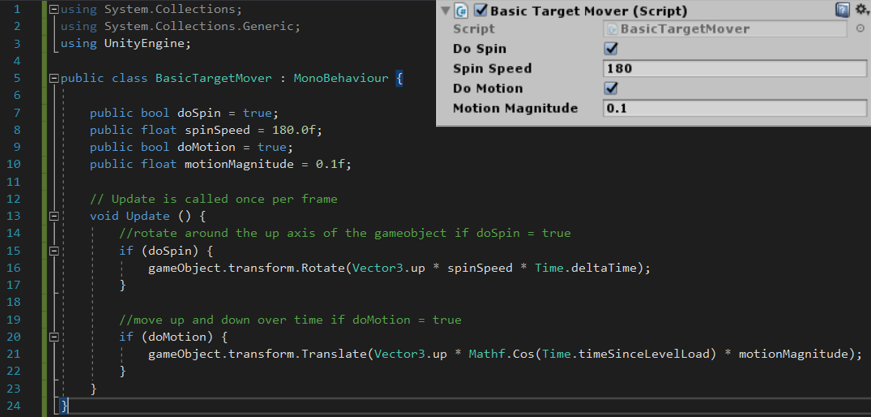
\includegraphics[width=\textwidth]{basic_target_mover_bool.png}\end{center}
\subsubsection{\texttt{enum} datatype and \texttt{switch} statements}
Up till now we can effectively switch on and off the individual motion components. But what if we have more than two types of motion? We can go on creating bool variables and if statements but that would make the component interface in Unity too complicated and cluttered. A better solution is to use the enumeration datatype.
\vspace{6pt} 

Let us check out the \texttt{TargetMover.cs} script we have in our assets directory. One disadvantage is that we can only choose one type of motion (i.e. spin and vertical motion cannot be switched on simultaneously).
\begin{center}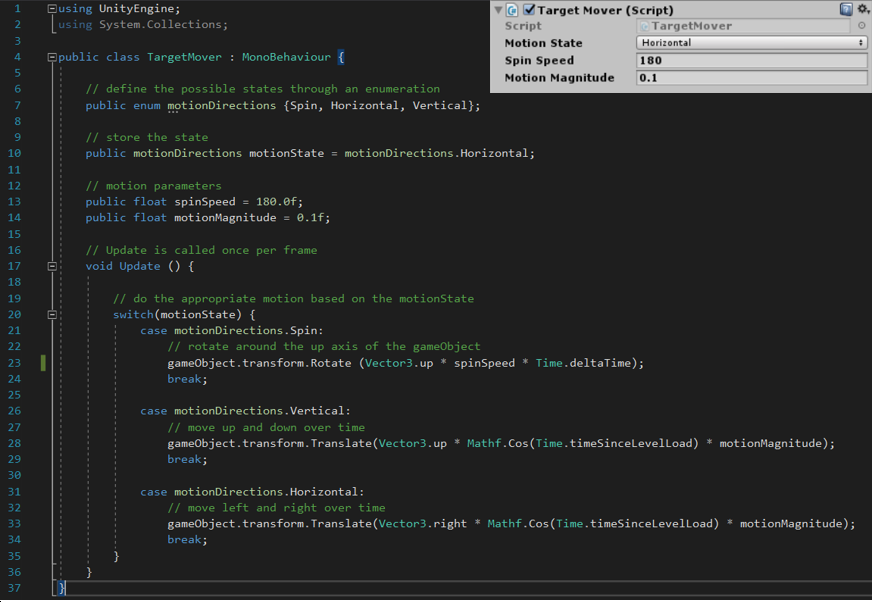
\includegraphics[width=\textwidth]{target_mover_enum.png}\end{center}
\pagebreak
Some points to note about this are:
\begin{itemize}
	\item \texttt{public enum motionDirections {Spin,Horizontal,Vertical}}: basically an array where we define a list of all possible motion states
	\item \texttt{public motionDirections motionState = motionDirections.Horizontal}: initializes the motion state to horizontal (can be changed in the editor)
	\item the \texttt{switch} statement:
	\begin{itemize}
		\item[$-$] \texttt{case motionDirections.Spin}: initializes a case which instructs the program to check whether or not \texttt{motionDirections.Spin} is true
		\item[$-$] every case must contain a \texttt{break} statement (so that the switch case breaks on the first occurrence of a satisfied case and ignores all further cases)
		\item[$-$] there can be an optional \texttt{default} case which runs if none of the cases are satisfied
	\end{itemize}
\end{itemize}
\subsection{Player, camera, projectiles and shooting}
\textit{(This section is currently in the works. Expect it to be up within a week's time.)}


\hrulefill
%\begin{center}\textbf{END OF COURSE DOCUMENTATION}\end{center}
%This is the end of the course documentation. Thank you for showing interest and reading till the end. If you have any suggestions for this or other documents, feel free to contact me using the links on my website.

%\hrulefill

\end{document}
